\documentclass[12pt]{report}

% \usepackage[utf8]{inputenc}
% \usepackage[T1]{fontenc}

% \usepackage[default]{fontsetup}
\usepackage{termes-otf}

% \usepackage{amsmath}
% \usepackage{amsthm}
% \usepackage{amssymb}

\usepackage[a4paper, margin=25mm]{geometry}

\usepackage{setspace} \onehalfspace

\usepackage[estonian]{babel}

\usepackage[hidelinks]{hyperref}

\usepackage{booktabs}

\usepackage{graphicx}

\usepackage{yquant} \useyquantlanguage{groups} \newcommand*{\yquanton}{}

\usepackage[sorting=none, style=ieee, maxbibnames=99]{biblatex}
\addbibresource{srcs.bib}

\def\paren#1{\left(#1\right)}
\def\sparen#1{\left[#1\right]}
\def\cparen#1{\left\{#1\right\}}

\def\abs#1{\left|#1\right|}

\def\d#1{\mathinner{d#1}}

\def\bra#1{\left<#1\right|}
\def\ket#1{\left|#1\right>}

\def\CNOT{\mathop{\rm CNOT}\nolimits}
\def\SWAP{\mathop{\rm SWAP}\nolimits}

\def\QFT{\mathop{\rm QFT}\nolimits}

\begin{document}

\begin{titlepage}
    \begin{center}
        \large
        {\sc Tartu Ülikool} \\
        Loodus- ja täppisteaduste valdkond \\
        Füüsika instituut \\


        \vspace{25mm}
        \Large Mattias Märka

        \vspace{4mm}
        \Huge Molekulaarse hamiltoniaani põhioleku energia leidmine faasi hindamise algoritmi abil

        \vspace{20mm}
        \Large Bakalaureusetöö (6 EAP) \\
        Füüsika, keemia ja materjaliteaduse õppekava \\
	Füüsika eriala \\

        \vspace{20mm}
        \begin{flushright}
            \Large Juhendaja: Veiko Palge, PhD
        \end{flushright}

        \vfill
        \large Tartu 2025
    \end{center}
\end{titlepage}

\newpage

\noindent\textbf{\large Molekulaarse hamiltoniaani põhioleku energia leidmine faasi hindamise algoritmi abil}

\vspace*{1ex}

\noindent\textbf{Lühikokkuvõte:}
Klassikaliste arvutitega saab täpselt simuleerida vaid lihtsamaid kvantsüsteeme, kuivõrd parim täpne klassikaline algoritm kuulub eksponentsiaalse keerukuse klassi.
Kvantarvutitega saab kvantsüsteemi simuleerimiseks kasutada faasi hindamise algoritmi, mille keerukus on aga kõigest polünoomne.
Sestap loodetakse kvantarvutitega tulevikus simuleerida klassikaliste arvutitega täpselt simuleerimiseks liialt keerulisi kvantsüsteeme.
Üks selliseid süsteeme, mille täpne simuleerimine võib käia klassikalistele arvutitele üle jõu, on molekuli elektronstruktuur.
Selles töös tutvustataksegi faasi hindamise algoritmil põhinevat meetodit elektronstruktuuri ülesande lahendamiseks, täpsemalt molekulaarse süsteemi põhienergia leidmiseks.
Meetodit rakendatakse lihtsa molekuli \(\rm H_2\) põhienergia leidmiseks.
Esmalt tutvustatakse elektronstruktuuri ülesande teoreetilist tausta.
Järgmisena antakse ülevaade molekulaarse süsteemi hamiltoniaani põhienergia leidmiseks vajalikest vahenditest: Jordan-Wigneri teisendusest, trotteriseerimisest, treppalgoritmist ja faasi hindamise algoritmist.
Arvutused viiakse läbi kasutades kvantarvuti klassikalist simulaatorit.
Lõpuks käsitletakse vajalike parameetrite valikut ja ülesande lahendamise võimalikkust kvantarvutil.

\vspace*{1ex}

\noindent\textbf{Võtmesõnad:}
kvantarvutus, kvantkeemia, kvantalgoritmid, faasi hindamise algoritm, elektronstruktuuri ülesanne

\vspace*{1ex}

\noindent\textbf{CERCS:}
P190 Matemaatiline ja üldine teoreetiline füüsika, klassikaline mehaanika, kvantmehaanika, relatiivsus, gravitatsioon, statistiline füüsika, termodünaamika;
P410 Teoreetiline ja kvantkeemia

\vspace*{5ex}

\noindent\textbf{\large Computation of the ground state energy of a molecular hamiltonian using the quantum phase estimation algorithm}

\vspace*{1ex}

\noindent\textbf{Abstract}:
The use of classical computers for exact simulation is limited to only the simplest quantum systems because even the best classical algorithms for this purpose belong to the exponential complexity class.
In contrast, quantum computers can utilize the quantum phase estimation algorithm of polynomial complexity.
Thus, it is believed that in the future quantum computers may be used to simulate quantum systems that are too complex to simulate using a classical computer.
The electronic structure problem of quantum chemistry is of particular interest.
This thesis gives an overview of a method based on the quantum phase estimation algorithm for solving the electronic structure problem, particularly calculating the ground state energy of a molecular system.
The method is used to calculate the ground state energy of the simple molecule \(\rm H_2\).
First, an introduction is given to the electronic structure problem.
Then, an overview is given of the quantum computational methods used to solve the problem: the Jordan-Wigner decomposition, trotterization, staircase algorithm, and phase estimation algorithm.
The quantum circuit is run on a classical computer using the statevector simulator.
Finally, the choice of simulation parameters and the possibility of using a quantum computer for the calculations is discussed.

\noindent\textbf{Keywords:}
quantum computing, quantum chemistry, quantum algorithms, quantum phase estimation algorithm, electronic structure problem

\vspace*{1ex}

\noindent\textbf{CERCS:}
P190 Mathematical and general theoretical physics, classical mechanics, quantum
mechanics, relativity, gravitation, statistical physics, thermodynamics; P410 Theoretical chemistry, quantum chemistry

\tableofcontents

\chapter{Sissejuhatus}

Kvantarvutuste valdkonna üks peamine arengumotivatsioon oli soov simuleerida keerulisi kvantsüsteeme.
Juba 1980ndatel, kui valdkond oli alles tekkimas, käisid Juri Manin ja Richard Feynman teineteisest eraldi välja idee, et kvantsüsteemide simuleerimiseks võiks hästi sobida just kvantarvuti~\cite{manin, feynman}.

Klassikaline simuleerimine on füüsikalise süsteemi käitumise uurimine arvutuslikult; kvantsimuleerimine on käitumise uurimine kvantarvutuslikult.
Simulatsiooniülesande saab analüütiliselt lahendada vaid lihtsaimate kvantsüsteemide jaoks, mille tuntuimad näited on harmooniline ostsillaator ja vesiniku aatom.
Keerukamate süsteemide klassikaliseks simuleerimiseks kasutatakse numbrilisi meetodeid~\cite{szabo+ostlund, whitfield+etal2011}.
Kvantsüsteemi simuleerimisülesande klassikaline lahendamine on aga möödapääsmatult kulukas: Schrödingeri võrrandi klassikalise lahendamise ressursikulu sõltub süsteemi suurusest eksponentsiaalselt~\cite{whitfield+etal2011, mcardle+etal, cao+etal, kassal+etal}.
Klassikaliselt ei pruugi suuremaid ülesandeid olla kunagi võimalik lahendada, ammugi täpselt, kuid neid võib olla võimalik lahendada kvantarvutuslikult.

Nimelt on teada mitu kvantalgoritmi, mille teoreetiline efektiivsus ületab klassikalise analoogi oma.
Komplekssusteoorias öeldakse, et lahenduvad on need ülesanded, mille ressursikulu sõltub süsteemi suurusest polünoomselt; lahendamatud on need ülesanded, mille ressursikulu sõltub süsteemi suurusest eksponentsiaalselt.
Mitmed klassikaliselt lahendamatud ülesanded on kvantarvutuslikult lahendatavad, nende hulgas ka kvantsüsteemide simuleerimise ülesanne.
Arvatakse, et kvantalgoritmidega saab tulevikus lahendada ülesandeid, mille klassikalist lahendamist peetakse jäädavalt liiga kulukaks.
Klassikalisest efektiivsemad kvantalgoritmid on võimalikud tänu kvantarvutuse ainulaadsetele vahenditele.

Siiani pole kvantarvututitega õnnestunud lahendada veel ühtegi sellist praktilise väärtusega probleemi, mida ei saa lahendada on klassikilaliselt.
Nimelt takistab kvantarvutite kasutamist nende ebatäiuslik riistvara: arvutusi segab kõrge müratase~\cite{whitfield+etal2022}.

Ent kvantalgoritme on mõttekas uurida tuleviku tarvis, sest kvantarvutite riistvara areneb pidevalt.
Pretsedendiks on klassikaliste arvutite kiire areng.
Lähemas tulevikus võib õnnestuda kasutada hübriidalgoritme, mis põhinevad kvantarvutite ja klassikaliste arvutite koostööl~\cite{omalley+etal}.

Käesoleva töö eesmärgiks on demonstreerida klassikalisest efektiivsemat kvantarvutuslikku meetodit molekulaarse hamiltoniaani simuleerimiseks.
See meetod põhineb faasi hindamise algoritmil.
Süsteemiks on vesiniku molekul \(\rm H_2\), ülesandeks on põhienergia leidmine kui näide elektronstruktuuri ülesandest.

Lahendamine algab klassikaliste eelarvutustega, mida tutvustab peatükk~\ref{chap:qchem}.
Eelarvutuste tulemuseks on hamiltoniaan teise kvantiseerimise kujul.
Peatükk~\ref{chap:qcomp} käsitleb ülesande kvantarvutuslikku lahendamist.
Sammud lahendamiseks on järgmised~\cite{whitfield+etal2011}.

\begin{enumerate}
    \item Teise kvantiseerimise kujul molekulaarne hamiltoniaan tuleb esitada kvantbittide ruumis, mis on teemaks jaotises~\ref{sec:jw}.
    \item Kvantbittide ruumis esitatud molekulaarse hamiltoniaani põhjal tuleb koostada ajalise arengu operaator ja realiseerida see kvantväravana, mida tutvustab jaotis~\ref{sec:qcirc}.
    \item Ajalise arengu operaatori omaväärtused tuleb leida kasutades faasi hindamise algoritmi, millest räägitakse lähemalt alapeatükis~\ref{sec:pea}.
\end{enumerate}
Selguse huvides on sammud tekstis esitatud vastupidises järjekorras võrreldes äsja tooduga.
Metoodikat, tulemusi ja edasiarendusi käsitleb peatükk~\ref{chap:results}.

\chapter{Elektronstruktuuri ülesanne}\label{chap:qchem}

Kuigi töös käsitletav kvantarvutuslik meetod sobib molekulaarse süsteemi mistahes omaoleku energia leidmiseks, siis piirdume käsitluse lihtsuse huivides siin töös põhioleku energia leidmisega.
Viimast kitsendust on eeldatud ka siin peatükis.
Põhioleku energia leidmiseks on tarvis teada, milline on elektronkatet iseloomustav hamiltoniaan \(H\).
Hiljem näeme, et samuti on vajalik põhioleku lainefunktsiooni $\Psi_0$ lähendus, kuid see ei pea olema täpne.
Selle peatüki teemaks ongi arvutused hamiltoniaani ja põhioleku lainefunktsiooni lähenduse leidmiseks.
Need arvutused on ülesande lahendamiseks vajalikud, kuid mitte töö põhiosa, sestap nimetame neid eelarvutusteks.
Peatükis on vaatluse all järgmised teemad.
Esiteks, alapeatükis~\ref{sec:molhamgen} esitame molekulaarse süsteemi hamiltoniaani üld\-kuju.
Järgmiseks, alapeatükis~\ref{sec:bornopen} lihtsustame seda hamiltoniaani Born-Oppenheimeri lähenduse abil.
Siis, alapeatükis~\ref{sec:hpsd} leiame lainefunktsiooni üldise kuju.
Edasi, alapeatükis~\ref{sec:hartfock} kasutame Hartree-Focki lähendust, et leida põhioleku lainefunktsiooni lähendus.
Viimaks, alapeatükis~\ref{sec:secquant} esitame ülesande teise kvantiseerimise kujul.
See peatükk põhineb peamiselt Szabo ja Ostlundi käsitlusel~\cite{szabo+ostlund}, aga ka Whitfieldi jt omal~\cite{whitfield+etal2011}.

\section{Molekulaarse hamiltoniaani üldkuju}\label{sec:molhamgen}

Molekulaarse süsteemi, milles on \(N\) elektroni ja \(M\) tuuma, hamiltoniaani üldkuju aatom\-ühikutes on
\begin{align}\label{eq:molham}
    H_\text{mol} =
    \underbrace{- \sum_{i = 1}^N \frac{1}{2} \nabla_i^2}_\text{(a)}
    \underbrace{- \sum_{A = 1}^M \frac{1}{2 M_A} \nabla_A^2}_\text{(b)}
    \underbrace{- \sum_{i = 1}^N \sum_{A = 1}^M \frac{Z_A}{r_{iA}}}_\text{(c)}
    \underbrace{+ \sum_{i = 1}^N \sum_{j > i}^N \frac{1}{r_{ij}}}_\text{(d)}
    \underbrace{+ \sum_{A = 1}^M \sum_{B > A}^M \frac{Z_A Z_B}{r_{AB}}}_\text{(e)} \rlap{,}
\end{align}
kus \(M_A\) on tuuma \(A\) ja elektroni massi suhe, \(Z_A\) on tuuma \(A\) aatomnumber, \(r_{ij}\) on elektronide \(i\) ja \(j\) vahekaugus ning \(R_{AB}\) on tuumade \(A\) ja \(B\) vahekaugus.
Kutsume hamiltoniaani~\eqref{eq:molham} edaspidi molekulaarseks hamiltoniaaniks.
Selles esinevad järgmised liikmed: (a) on elektronide kineetilise energia liige, (b) on tuumade kineetilise energia liige, (c) on elektronide ja tuumade tõmbumise liige, (d) on elektronide omavahelise tõukumise liige ja (e) on tuumade omavahelise tõukumise liige.

Üldine hamiltoniaan~\eqref{eq:molham} kirjeldab nii elektronide kui ka tuumade dünaamikat, kuid elektronstruktuuri ülesande seisukohalt huvitab meid vaid elektronide dünaamika.
Eeldusel, et tuumade dünaamika pole oluline, on võimalik hamiltoniaani~\eqref{eq:molham} oluliselt lihtsustada, mida käsitlebki järgmine alapeatükk~\ref{sec:bornopen}.

\section{Born-Oppenheimeri lähendus}\label{sec:bornopen}

Et tuumade massid on palju suuremad kui elektronide massid, siis liiguvad tuumad palju aeglasemalt kui elektronid.
Kvantkeemias kasutatakse laialdaselt Born-Oppenheimeri lähendust, mille järgi on tuumad paigal.
Kasutame seda lähendust ka siin töös.

Born-Oppenheimeri lähendus lubab molekulaarset hamiltoniaani~\eqref{eq:molham} lihtsustada.
Esiteks võib arvestamata jätta tuumade kineetilise energia liikme (b), sest see on ligikaudu null.
Teiseks võib arvestamata jätta tuumade omavahelise tõmbumise liikme (e), sest see on konstantne.
Tulemuseks on vaid elektronide dünaamikat kirjeldav hamiltoniaan
\begin{align}\label{eq:elham}
    H_\text{elek} =
    \underbrace{- \sum_{i = 1}^N \frac{1}{2} \nabla_i^2}_\text{(a)}
    \underbrace{- \sum_{i = 1}^N \sum_{A = 1}^M \frac{Z_A}{r_{iA}}}_\text{(c)}
    \underbrace{+ \sum_{i = 1}^N \sum_{j > i}^N \frac{1}{r_{ij}}}_\text{(d)} \rlap{,}
\end{align}
mida kutsume elektrooniliseks hamiltoniaaniks.
Konstantse liikme~(e) arvestamata jätmise tõttu erinevad elektrooniline hamiltoniaan~\eqref{eq:elham} ja molekulaarne hamiltoniaan~\eqref{eq:molham} küll omaväärtuste poolest, kuid mitte omafunktsioonide poolest.
Täpsemalt öeldes kehtib seos
\begin{align}\label{eq:eigenelvsmol}
    E_\text{mol} = E_\text{elek} + E_\text{tuum} \rlap{,}
\end{align}
kus \(E_\text{mol}\) ja \(E_\text{elek}\) on vastavalt molekulaarse hamiltoniaani~\eqref{eq:molham} ja elektroonilise hamiltoniaani~\eqref{eq:elham} omaväärtused mingi ühise omafunktsiooni jaoks	 ning \(E_\text{tuum}\) on kõikide omafunktsioonide jaoks sama konstant.
Füüsikaliselt tähendab viimane võrdus seda, et Born-Oppenheimeri lähenduses erineb elektronkatte energia molekuli energiast konstantse tuumade energia võrra.
Edaspidi jätame ära alaindeksi ``elek'', kuivõrd meid huvitabki vaid elektronkate.

\section{Hartree korrutis ja Slateri determinant}\label{sec:hpsd}

Hamiltoniaan~\eqref{eq:elham} ei võta arvesse spinni.
Kuid, kuna me soovime spinni arvestada, siis peame selle lainefunktsioonile lisama.
Lainefunktsioonile \(\Psi\) ongi kaks tingimust.
Ühest küljest peab see rahuldama Schrödingeri võrrandit.
Teisalt peab see rahuldama antisümmeetria printsiipi
\begin{align}\label{eq:antisim}
    \Psi(\vec{x}_1, \ldots, \vec{x}_i, \ldots, \vec{x}_j, \ldots, \vec{x}_N) =
    -\Psi(\vec{x}_1, \ldots, \vec{x}_j, \ldots, \vec{x}_i, \ldots, \vec{x}_N) \rlap{,}
\end{align}
kus \(\vec{x}_1\), \(\ldots\), \(\vec{x}_N\) on elektronide \(1\), \(\ldots\), \(N\) üldised koordinaadid.
Üldine kordinaat on
\begin{align}
    \vec{x} = (\vec{r}, \omega) \rlap{,}
\end{align}
kus \(\vec{r}\) on ruumiline kordinaat ja \(\omega\) spinn.
Jämedalt öeldes on antisümmeetria printsiip oluline, kuna see on Pauli keeluprintsiibi üldisem sõnastus.

Sobivate omadustega lainefunktsiooni saab molekulaarorbitaalide teooriast.
Selles teoorias nimetatakse spinnorbitaaliks funktsiooni
\begin{align}\label{eq:spinorb}
    \chi_i(\vec{x}) = \begin{cases}
        \alpha(\omega) \phi_i(\vec{r})\text{,} & \text{kui \(i\) ei jagu \(2\)-ga} \rlap{,}\\
        \beta(\omega) \phi_{i-1}(\vec{r})\text{,} & \text{kui \(i\) jagub \(2\)-ga} \rlap{.} \\
    \end{cases}
\end{align}
Spinnorbitaali võib tõlgendada ühe elektroniga molekulaarse süsteemi lainefunktsioonina.
Funktsioon \(\alpha(\omega)\) vastab spinn-alla seisundile ja funktsioon \(\beta(\omega)\) spinn-üles seisundile.
Funktsioonid \(\cparen{\phi_j \middle| j = 1,2, \ldots, K}\) on ruumilised orbitaalid (mis ei arvesta spinni).
Iga ruumilise orbitaali kohta on kaks spinn\-orbitaali.
Spinnorbitaalide korrutist
\begin{align}
    \Psi^\text{HP}(\vec{x}_1, \vec{x}_2, \cdots, \vec{x}_N) =
    \chi_i(\vec{x}_1) \chi_j(\vec{x}_2) \cdots \chi_k(\vec{x}_N)
\end{align}
nimetatakse Hartree korrutiseks.
Hartree korrutis on \(N\)-i teineteisega mitteinterakteeruva elektroni süsteemi lainefunktsioon, mis antisümmeetria printsiipi ei arvesta.
Selle järgi on elektronid sõltumatud: süsteemi hamiltoniaani saab kirja panna kujul
\begin{align}
    H = \sum_i^N h(i) \rlap{,}
\end{align}
kus \(h(i)\) on üksiku elektroni hamiltoniaan.
Et kehtib
\begin{align}
    E = \sum_j^N \epsilon_j \rlap{,}
    \qquad \text{kus} \qquad
    H \Psi^\text{HP} = E \Psi^\text{HP}
    \quad \text{ja} \quad
    h(i) \chi_j(\vec{x_i}) = \epsilon_j \chi_j(\vec{x_i}) \rlap{,}
\end{align}
siis sellise süsteemi koguenergia on üksikute elektronide energiate summa, mis näitabki Hartree korrutise sobivust lainefunktsiooniks mitme elektroniga süsteemi lihtsustatud juhul.

Antisümmeetria printsiipi ja elektronide vastasmõju arvestab Slateri determinant
\begin{align}\label{eq:slater}
    \Psi(\vec{x_1}, \vec{x_2}, \ldots, \vec{x_n}) =
    \frac{1}{\sqrt{N!}} \begin{vmatrix}
        \chi_i(\vec{x_1}) & \chi_j(\vec{x_2}) & \cdots & \chi_k(\vec{x_2}) \\
        \chi_i(\vec{x_2}) & \chi_j(\vec{x_2}) & \cdots & \chi_k(\vec{x_2}) \\
        \vdots & \vdots & & \vdots \\
        \chi_i(\vec{x_N}) & \chi_j(\vec{x_N}) & \cdots & \chi_k(\vec{x_N}) \\
    \end{vmatrix} \rlap{.}
\end{align}
Slateri determinant on füüsikaliselt sobiv elektrooniline lainefunktsioon: saab näidata, et see võtab arvesse antisümmeetria printsiipi.

\section{Hartree-Focki lähendus}\label{sec:hartfock}

Kui hamiltoniaan~\eqref{eq:molham} on arvutamiseks liiga keeruline, siis kasutatakse klassikalises kvantkeemias arvutusressursside kokku hoidmiseks Hartree-Focki lähendust.
Selles töös on Hartree-Focki lähendus vajalik vaid eelarvutuste läbiviimiseks: see lähendus lubab leida spinnorbitaalid \(\cparen{\chi_j | j=1, 2, \ldots, 2K}\), mis on vajalikud teise kvantiseerimise kuju leidmiseks, nagu selgub järgmises alapeatükis~\ref{sec:secquant}.

Hamiltoniaan~\ref{eq:molham} puhul on tegu mitme keha probleemiga.
Ülesande lihtsustamiseks eeldatakse Hartree-Focki lähenduses, et iga elektron liigub efektiivses väljas, mis saadakse teiste elektronide mõjude keskmistamisel.
Matemaatiliselt tähendab see järgmist.

Elektroonilise lainefunktsiooni üldkuju on~\eqref{eq:slater}.
Põhioleku lainefunktsioon on \(\Psi_0\) selline, mille energia
\begin{align}
    E_0 = \bra{\Psi_0} H \ket{\Psi_0}
\end{align}
on minimaalne.
Energia väärtus sõltub spinnorbitaalide valikust.
Minimeerimine viib Hartree-Focki võrrandini
\begin{align}
    f(i) \chi(\vec{x}_i) = \epsilon \chi(\vec{x}_i) \rlap{,}
\end{align}
kus
\begin{align}
  f(i) = -\frac{1}{2} \nabla_i^2 - \sum_{A = 1}^M \frac{Z_A}{r_{iA}} + v^\text{HF}(i)
\end{align}
on Focki operaator.
Liige \(v^\text{HF}\) on keskmine potentsiaal, mida kogeb üks elektron teiste elektronide tõttu.
Lahendamise tulemuseks on Hartree-Focki spinnorbitaalide komplekt \(\cparen{\chi_i \middle| i = 1, 2, \ldots}\), millele vastab energiate komplekt \(\cparen{\epsilon_i \middle| i = 1, 2, \ldots}\).

Neid \(N\)-i spinnorbitaali, mis lainefunktsioonis esinevad, nimetatakse täidetud orbitaalideks; neid, mis ei esine, nimetatakse täitmata orbitaalideks.
Meie jaoks on oluline, et põhiolekus on täidetud vaid madalaima energiaga orbitaalid.

Hartree-Focki võrrandil on lõpmata palju lahendeid: tulemuseks on lõpmata palju spinnorbitaale.
Praktikas valitakse arvutamiseks siiski lõpliku suurusega baasifunktsioonide komplekt $\cparen{\phi_i \middle| i = 1, 2, \ldots, K}$, mille tulemusena saadakse lõplik arv spinnorbitaale.
Baasifunktsioonide komplekti nimetatakse keemiliseks baasiks, kusjuures baasi valik on üks elektronstruktuuri arvutuste olulisi eeldusi.
Piirangud valikus seab ülesande keerukus: suuremad baasid annavad täpsemad tulemused, ent arvutused nendega on kulukamad.

\section{Teine kvantiseerimine}\label{sec:secquant}

Kvantkeemias kasutatakse arvutamiseks tihti teise kvantiseerimise kuju, milles lainefunktsiooni esitus on kompaktsem.
Selles töös on oluline, et teise kvantiseerimise kuju on vajalik lainefunktsiooni kujutamiseks kvantbittide ruumi, mis on teemaks alapeatükis~\ref{sec:jw}.

Teise kvantiseerimise formalismis esitatakse lainefunktsioon täitearvude esituses
\begin{align}
    \Psi(\vec{x}_1, \vec{x}_2, \ldots, \vec{x}_N) =
    \ket{\chi_1 \chi_2 \cdots \chi_{2K}} \rlap{,}
\end{align}
kus \(\chi \in \cparen{0, 1}\) viitab vastavalt täitmata või täidetud orbitaalile.
Selline lainefunktsiooni esitus on kompaktsem kui esitus Slateri determinandina, kuid antisümmeetria printsiibi kehtimisele tuleb pöörata eraldi tähelepanu.

Teise kvantiseerimise formalismis võetakse antisümmeetria printsiipi arvesse algebraliselt.
Selleks defineeritakse kaks sobivate omadustega operaatorit: tekkeoperaator \(a_i^\dagger\) ja kaooperaator \(a_i\).
Tekkeoperaator \(a_i^\dagger\) tekitab süsteemi juurde elektroni spinnorbitaalile \(\chi_i\):
\begin{align}
    a_i^\dagger \ket{\chi_k \cdots \chi_l} = \ket{\chi_i \chi_k \cdots \chi_l} \rlap{.}
\end{align}
Kaooperaator \(a_i\) eemaldab süsteemist elektroni spinnorbitaalilt \(\chi_i\):
\begin{align}
    a_i \ket{\chi_i \chi_k \cdots \chi_l} = \ket{\chi_k \cdots \chi_l}\rlap{.}
\end{align}
Kehtivad kommutatsioonireeglid
\begin{align}\label{eq:comrules}
    \sparen{a_i^\dagger, a_j^\dagger} = 0 \rlap{,}
    \qquad \sparen{a_i, a_j} = 0 \rlap{,}
    \qquad \sparen{a_i, a_j^\dagger} = \delta_{ij} \rlap{.}
\end{align}

Tekke- ja kaoperaatorite kaudu saab hamiltoniaani esitada teise kvantiseerimise kujul järgmiselt,
\begin{align}
    H = \sum_{pq}h_{pq}a_p^\dagger a_q
    + \frac{1}{2} \sum_{pqrs} a_p^\dagger a_q^\dagger a_r a_s \rlap{,}
\end{align}
kus
\begin{align}\label{eq:molint1}
    h_{pq} = \int\d{\vec{x}_i} \chi_p^*(\vec{x}_i)
    \paren{-\frac{1}{2} \nabla^2 - \sum_A \frac{Z_a}{r_{iA}}} \chi_q(\vec{x}_i)
\end{align}
on ühe keha operaatori maatrikselement ja
\begin{align}\label{eq:molint2}
    h_{pqrs} = \int \d{\vec{x}_1} \d{\vec{x}_2}
    \frac{\chi_p^*(\vec{x}_1) \chi_q^*(\vec{x}_2) \chi_r(\vec{x}_2) \chi_s(\vec{x}_1)}{r_{12}}
\end{align}
on kahe keha operaatori maatrikselement.
Nimetame suurusi \eqref{eq:molint1} ja \eqref{eq:molint2} molekulaarseteks integraalideks, sest need seovad hamiltoniaani esimese ja teise kvantiseerimise kuju.
Need integraalid saab arvutada klassikaliselt ja need on põhienergia leidmise ülesande esimeseks eelarvutuseks. Teine eelarvutus on Jordan-Wigneri teisendus, mis on teemaks järgmises peatükis.

\chapter{Kvantarvutuslik lahendamine}\label{chap:qcomp}

See peatükk annab ülevaate molekulaarse süsteemi põhienergia kvantarvutuslikust leidmisest.
Esimene alapeatükk~\ref{sec:terms} käsitleb kvantarvutuse põhitõdesid.
Teise alapeatüki~\ref{sec:pea} teemaks on faasi hindamise algoritm ise.
Kolmas alapeatükk~\ref{sec:hamsim} räägib hamiltoniaani simuleerimisest kvantahelana.
Alapeatükid~\ref{sec:terms} ja~\ref{sec:pea} toetuvad Nielseni ja Chuangi~\cite{nielsen+chuang}; Kaye, Laflamme'i ja Mosca~\cite{kaye+laflamme+mosca} ning Whitfield jt~\cite{whitfield+etal2011} käsitlusele.
Alpeatüki~\ref{sec:hamsim} viited on teksti sees.

\section{Põhimõisted}\label{sec:terms}

Selles töös kasutame kvantarvutuse ahelamudelit, mille põhimõisted on kvantbitt ja kvantvärav.
Kvantahelamudel sarnaneb üldpildis klassikalisele ahelamudelile.
Järgneb kvantahelamudeli lühike ülevaade rõhutamaks mõnesid erinevusi.

Kvantarvutuses on informatsiooni põhiühikuks kvantbitt, mis on Hilberti ruumi objekt.
Kõik kvantbiti olekud saab kirja panna kujul
\begin{align}
    \ket{\phi} = \alpha \ket{0} + \beta \ket{1} \rlap{,}
    \qquad \alpha, \beta \in \mathbb{C} \rlap{,}
    \qquad \abs{\alpha}^2 + \abs{\beta}^2 = 1 \rlap{,}
\end{align}
kus
\begin{align}\label{eq:compbasis}
    \ket{0} = \begin{pmatrix}
        1 \\
        0 \\
    \end{pmatrix} \rlap{,}
    \qquad
    \ket{1} = \begin{pmatrix}
        0 \\
        1 \\
    \end{pmatrix} \rlap{,}
\end{align}
on ortonormaalsed vektorid.
Kvantarvutuse kontekstis kastutakse kokkuleppeliselt Pauli \(Z\) operaatori omabaasi, mida nimetatakse arvutuslikuks baasiks.

Kvantbittide kogumit nimetatakse kvantregistriks ja selle olekuruum on üksikuid kvantbitte iseloomustavate Hilberti ruumide tensorkorrutis.
Kvantregistri jaoks on võimalikud kahte moodi olekud: korrutisolekud ja põimitud olekud.
Korrutisolekus saab lahutada üksikute kvantbittide olekuteks:
\begin{align}
    \ket{\Phi}
    = \ket{\phi_1} \otimes \ket{\phi_2} \otimes \cdots
    = \ket{\phi_1 \phi_2 \cdots} \rlap{,}
\end{align}
Põimitud olekut ei saa lahutada üksikute bittide olekuteks:
\begin{align}
    \ket{\Phi}
    \ne \ket{\phi_1 \phi_2 \cdots} \rlap{,}
\end{align}
Näide põimitud olekust on Belli olek
\begin{align}
    \frac{\ket{00} + \ket{11}}{\sqrt 2} \rlap{.}
\end{align}
Klassikalises teoorias põimitust ei esine.

Kvantväravad sooritavad kvantbittidel unitaarsed operatsioone.
Need võivad mõjutada ühte või rohkemat kvantbitti.
Mitut kvantbitti mõjutavad väravad võivad olla põimivad.
Siin töös kasutatud ühekvantbitised väravad on toodud tabelis~\ref{tab:gates}.
Võimalikke kvantväravaid on küll lõpmata palju, kuid riistvaras on vaja realiseerida vaid mõned väravad, mis moodustavad universaalse komplekti.
Kõik teised väravad saab esitada universaalse komplekti kaudu.
Universaalseid komplekte on lõpmata palju, ent komplektis peab alati olema vähemalt üks põimiv värav.
Antud töös kasutatakse põimimiseks juhitud eituse väravat.
Juhitud väravad on sellised, mis rakenduvad sihtkvantbitile vaid siis, kui juhtkvantbitt on olekus \(\ket1\), juhtkvantbitti muutmata.
Näide juhitud eituse rakendamisest on järgmine,
\begin{align}
    \CNOT \paren{\alpha \ket{0} \otimes \ket{1} + \beta \ket{1} \otimes \ket{1}}
    = \alpha \ket{0} \otimes \ket{1} + \beta \ket{1} \otimes \ket{0} \rlap{,}
\end{align}
kus tensorkorrutise vasakul on juhtkvantbitt ja paremal sihtkvantbitt.
Töös kasutatud juhitud väravaid pole enamasti tabelis~\ref{tab:gates} eraldi toodud.
Kvantahela osaks võib muidugi olla ka mõõtmine, ent see pole unitaarne operatsioon, mistõttu ei saa seda nimetata väravaks.
Siiski tähistatakse ahelates seda väravatega sarnaselt.

\begin{table}[]
    \centering
    \begin{tabular}{||c|c|c||}
        \toprule
        Operaator  & Maatriks & Tähis kvantahelas \\
        \midrule
        Pööre \(z\)-telje ümber \(R_z(\theta)\) & \(
        \begin{pmatrix}
            e^{-i\frac{\theta}{2}} & 0 \\
            0 & e^{i\frac{\theta}{2}} \\
        \end{pmatrix}
        \) & \lower6pt\hbox{
        \ifdefined\yquanton
        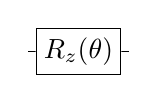
\begin{tikzpicture}
            \begin{yquant}
                qubit {} q[1];
                box {\(R_z(\theta)\)} q[0];
            \end{yquant}
        \end{tikzpicture}
        \fi} \\[1em]
        Faasinihe \(P(\lambda)\) & \(
        \begin{pmatrix}
            1 & 0 \\
            0 & e^{i\lambda} \\
        \end{pmatrix}
        \) & \lower6pt\hbox{
        \ifdefined\yquanton
        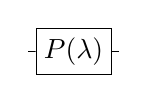
\begin{tikzpicture}
            \begin{yquant}
                qubit {} q[1];
                box {\(P(\lambda)\)} q[0];
            \end{yquant}
        \end{tikzpicture}
        \fi} \\[1em]
        Globaalse faasi nihe \(GP(\lambda)\) & \(
        \begin{pmatrix}
            e^{i\lambda} & 0 \\
            0 & e^{i\lambda} \\
        \end{pmatrix}
        \) & \lower6pt\hbox{
        \ifdefined\yquanton
        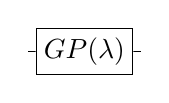
\begin{tikzpicture}
            \begin{yquant}
                qubit {} q[1];
                box {\(GP(\lambda)\)} q[0];
            \end{yquant}
        \end{tikzpicture}
        \fi} \\[1em]
        Juhitud eitus \(\CNOT\) & \(
        \begin{pmatrix}
            1 & 0 & 0 & 0 \\
            0 & 0 & 0 & 1 \\
            0 & 0 & 1 & 0 \\
            0 & 1 & 0 & 0 \\
        \end{pmatrix}
        \) & \lower6pt\hbox{
        \ifdefined\yquanton
        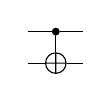
\begin{tikzpicture}
            \begin{yquant}
                qubit {} ctrl;
                qubit {} trgt;
                cnot trgt | ctrl;
            \end{yquant}
        \end{tikzpicture}
        \fi} \\
        Pauli \(X\) & \(
        \begin{pmatrix}
            0 & 1 \\
            1 & 0 \\
        \end{pmatrix}
        \) & \lower6pt\hbox{
        \ifdefined\yquanton
        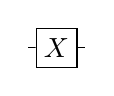
\begin{tikzpicture}
            \begin{yquant}
                qubit {} q[1];
                box {\(X\)} q[0];
            \end{yquant}
        \end{tikzpicture}
        \fi} \\[1em]
        Pauli \(Y\) & \(
        \begin{pmatrix}
            0 & -i \\
            i & 0 \\
        \end{pmatrix}
        \) & \lower6pt\hbox{
        \ifdefined\yquanton
        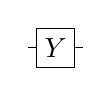
\begin{tikzpicture}
            \begin{yquant}
                qubit {} q[1];
                box {\(Y\)} q[0];
            \end{yquant}
        \end{tikzpicture}
        \fi} \\[1em]
        Pauli \(Z\) & \(
        \begin{pmatrix}
            1 & 0 \\
            0 & -1 \\
        \end{pmatrix}
        \) & \lower6pt\hbox{
        \ifdefined\yquanton
        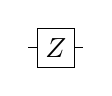
\begin{tikzpicture}
            \begin{yquant}
                qubit {} q[1];
                box {\(Z\)} q[0];
            \end{yquant}
        \end{tikzpicture}
        \fi} \\[1em]
        Hadamardi operaator \(H\) & \(
        \frac{1}{\sqrt{2}} \begin{pmatrix}
            1 & 1 \\
            1 & -1 \\
        \end{pmatrix}
        \) & \lower6pt\hbox{
        \ifdefined\yquanton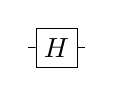
\begin{tikzpicture}
            \begin{yquant}
                qubit {} q[1];
                box {\(H\)} q[0];
            \end{yquant}
        \end{tikzpicture}
        \fi} \\[1em]
        Faasioperaator \(S\) & \(
        \begin{pmatrix}
            1 & 0 \\
            0 & i \\
        \end{pmatrix}
        \) & \lower6pt\hbox{
        \ifdefined\yquanton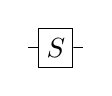
\begin{tikzpicture}
            \begin{yquant}
                qubit {} q[1];
                box {\(S\)} q[0];
            \end{yquant}
        \end{tikzpicture}
        \fi} \\[1em]
        Pöördfaasioperaator \(S^{\dagger}\) & \(
        \begin{pmatrix}
            1 & 0 \\
            0 & -i \\
        \end{pmatrix}
        \) & \lower6pt\hbox{
        \ifdefined\yquanton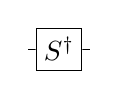
\begin{tikzpicture}
            \begin{yquant}
                qubit {} q[1];
                box {\(S^{\dagger}\)} q[0];
            \end{yquant}
        \end{tikzpicture}
        \fi} \\[1em]
        Bittide vahetus \(\SWAP\) & \(
        \begin{pmatrix}
            1 & 0 & 0 & 0 \\
            0 & 0 & 1 & 0 \\
            0 & 1 & 0 & 0 \\
            0 & 0 & 0 & 1 \\
        \end{pmatrix}
        \) & \lower6pt\hbox{
        \ifdefined\yquanton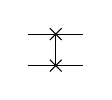
\begin{tikzpicture}
            \begin{yquant}
                qubit {} q[2];
                swap (q[0, 1]);
            \end{yquant}
        \end{tikzpicture}
        \fi} \\
        \midrule
        Mõõtmine & --- & \lower6pt\hbox{
        \ifdefined\yquanton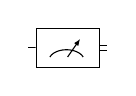
\begin{tikzpicture}
            \begin{yquant}
                qubit {} q[1];
                measure q[0];
            \end{yquant}
        \end{tikzpicture}
        \fi} \\
        \bottomrule
    \end{tabular}
    \caption{Töös kasutatud operaatorid, nende definitsioonid maatriksina ja tähistused ahelas.}
    \label{tab:gates}
\end{table}

Kvantäravate järjestuse ja bittidele rakendamise korra määrab kvantahel.
Joonisel~\ref{fig:circuits} on näide kvantahelast, mille lugemiseks tuleb arvestada järgmist.
Igat üksikut kvantbitti või -registrit tervikuna tähistab horisontaalne traat.
Traadist vasakul on sisend- ja paremal väljundolekud, kui need on olulised.
Operaatoreid tähitavad kastid.
Operaator rakendub igale kavantbitile, mille traat kasti läbib.
Katsutid~--- otspunktiga lõppevad vertikaalsed jooned~--- ühendavad operaatoreid juhtkvantbitile või juhtkvantregistritega, kui neid on.

\begin{figure}
    \centering
    \ifdefined\yquanton
    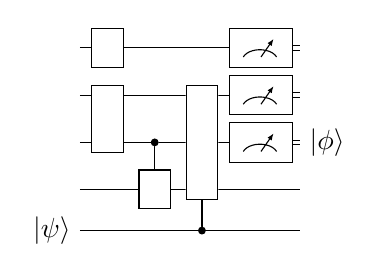
\begin{tikzpicture}
        \begin{yquant}
            qubit {} q[4];
            qubit {\(\ket{\psi}\)} q[+1];
            box {} q[0];
            box {} (q[1, 2]);
            box {} q[3] | q[2];
            box {} (q[1, 2, 3]) | q[4];
            measure q[0, 1, 2];
            output {\(\ket{\phi}\)} q[2];
        \end{yquant}
    \end{tikzpicture}
    \fi
    \caption{Näide kvantahelast.}
    \label{fig:circuits}
\end{figure}

\section{Faasi hindamise algoritm}\label{sec:pea}

Siin alapeatükis näitame, kuidas faasi hindamise algoritmi abil saab hinnata kvantbittide ruumis esitatud hamiltoniaani \(H\) omaväärtusi.
Esmalt, jaotises~\ref{sec:qftdef} tutvustama kvantarvutuslikku Fourier' teisendust ja pöördteisendust, mis on faasi hindamise algoritmi tähtsad osad.
Järgmisena, jaotises~\ref{sec:unit} näitame, kuidas faasi hindamise algoritmiga on võimalik leida unitaarse operaatori omaväärtusi.
Viimaks, jaotises~\ref{sec:ham} kasutame faasi hindamise algoritmi hamiltoniaani omaväärtuste leidmiseks.

\subsection{Kvantarvutuslik Fourier' teisendus ja pöördteisendus}\label{sec:qftdef}

Võtame vaatluse alla kvantarvutusliku Fourier' teisenduse ja pöördteisenduse algoritmid, mis on faasi hindamise algoritmi tähtsad osad.

Kvantarvutusliku Fourier' teisenduse definitsioon on
\begin{align}\label{eq:qftdef}
    \QFT\colon
    \ket{j} \mapsto \frac{1}{\sqrt{2^n}} \sum_{k=0}^{2^n-1} e^{2\pi ijk/2^n} \ket{k} \rlap{,}
\end{align}
kus \(\ket{j}\) ja \(\ket{k}\) \(n\)-kvantbitised baasivektorid.
Et tegemist on lineaarse operatsiooniga, siis piisab, kui käsitleda selle mõju baasivektoritele.

\begin{figure}
    \centering
    \ifdefined\yquanton
    \begin{tikzpicture}[scale=0.8]
        \begin{yquant}
            qubit {\(\ket{j_1}\)} q[1];
            qubit {\(\ket{j_2}\)} q[+1];
            qubit {\(\vdots\)} q[+1]; discard q[2];
            qubit {\(\ket{j_{n-1}}\)} q[+1];
            qubit {\(\ket{j_n}\)} q[+1];
            h q[0];
            box {\(P(2\pi/2^2)\)} q[0] | q[1];
            text {\(\ \ldots\ \)} q[0, 1, 3, 4];
            h q[1];
            text {\(\ \ldots\ \)} q[0, 1, 3, 4];
            box {\(P(2\pi/2^{n-2})\)} q[1] | q[3];
            box {\(P(2\pi/2^{n-1})\)} q[1] | q[4];
            text {\(\ \ldots\ \)} q[0, 1, 3, 4];
            h q[3];
            box {\(P(2\pi/2^2\)} q[3] | q[4];
            h q[4];
            swap (q[0, 4]);
            swap (q[1, 3]);
            output {\(\frac{\ket0+e^{2\pi0.j_n}\ket1}{\sqrt{2}}\)} q[0];
            output {\(\frac{\ket0+e^{2\pi0.j_{n-1}j_n}\ket1}{\sqrt{2}}\)} q[1];
            output {\(\vdots\)} q[2];
            output {\(\frac{\ket0+e^{2\pi0.j_2\cdots j_n}\ket1}{\sqrt{2}}\)} q[3];
            output {\(\frac{\ket0+e^{2\pi0.j_1\cdots j_n}\ket1}{\sqrt{2}}\)} q[4];
        \end{yquant}
    \end{tikzpicture}
    \fi
    \caption{Kvantarvutusliku Fourier' teisenduse ahel.}
    \label{fig:qft}
\end{figure}

Näitame, et kvantarvutusliku Fourier' teisenduse realiseerib ahel joonisel~\ref{fig:qft}.
Selleks on ilmekas kasutada tähistust
\begin{multline}
    j_1j_2\cdots j_n.j_{n+1}j_{n+2}\cdots j_m \\
    = j_1 2^{n-1} j_2 2^{n-2} + \cdots + j_n 2^0 + j_{n+1} 2^{-1} j_{n+2} 2^{-2} + \cdots j_m 2^{-m} \rlap{,}
    \qquad j_i \in \{0, 1\} \rlap{.}
\end{multline}
Teisisõnu, selles ja järgmises jaotises on komaga arvud kahendmurrud, mitte kümnendmurrud.
Edasises on veel vaja teada, et Hadamardi operaatori mõju baasvektoritele on
\begin{align}
    H\ket{0} = \frac{\ket{0} + \ket{1}}{\sqrt{2}}
    \qquad\text{ja}\qquad
    H\ket{1} = \frac{\ket{0} - \ket{1}}{\sqrt{2}} \rlap{.}
\end{align}
Viimased kaks tingimust saab kokku võtta üheks
\begin{align}\label{eq:hprop}
    H\ket{j_i} = \frac{\ket{0} + e^{2\pi i0.j_i}\ket{1}}{\sqrt{2}}\rlap{.}
\end{align}
Samuti on vaja teada, et faasioperaatori mõju baasivektoritele on
\begin{align}
    P(\lambda)\ket{0} = \ket{0}
    \qquad\text{ja}\qquad
    P(\lambda)\ket{1} = e^{i\lambda}\ket{1} .
\end{align}
Viimasest kahest tingimusest järeldub kasulik omadus
\begin{align}\label{eq:phaseprop}
    P(2\pi i0.0j_2)\paren{\frac{\ket{0} + e^{2\pi i 0.j_1} \ket{1}}{\sqrt{2}}}
    = \frac{\ket{0}+e^{2\pi i0.j_1j_2}\ket{1}}{\sqrt{2}} .
\end{align}
Järgime nüüd joonise~\ref{fig:qft} ahelat samm-sammult.
Ahela alguses on kvantbitid olekus
\begin{align}
    \ket{j_1} \otimes \ket{j_2} \otimes \cdots \otimes \ket{j_n} \rlap{.}
\end{align}
Esimeses etapis rakendatakse esimesele kvantbitile Hadamardi operaatorit \(H\) ja seejärel faasioperaatoreid \(P(2\pi/2^2)\), \(P(\pi/2^3)\), \(\ldots\), \(P(\pi/2^4)\) juhinduvalt vastavalt teisest, kolmandast, \(\ldots\), \(n\)-ndast kvantbitist.
Hadamardi operaatori \(H\) rakendamise järel on olek
\begin{align}
    \frac{\ket{0} + e^{2\pi i0.j_1}\ket{1}}{\sqrt{2}} \otimes \ket{j_2} \otimes \cdots \otimes \ket{j_n}
\end{align}
tulenevalt valemist~\eqref{eq:hprop}.
Faasioperaatori \(P(2\pi/2^2) = P(2\pi0.01)\) rakendamise järel juhinduvalt teisest kvantbitist on olek
\begin{align}
    \begin{cases}
        \frac{\ket{0} + e^{2\pi i0.j_1}\ket{1}}{\sqrt{2}} \otimes \ket{j_2} \otimes \cdots \otimes \ket{j_n}\text{,} & \text{kui \(j_2 = 0\)} \rlap{,} \\
        \frac{\ket{0} + e^{2\pi i0.j_11}\ket{1}}{\sqrt{2}} \otimes \ket{j_2} \otimes \cdots \otimes \ket{j_n}\text{,} & \text{kui \(j_2 = 1\)} \rlap{,} \\
    \end{cases}
\end{align}
tulenevalt valmist~\eqref{eq:phaseprop}.
Viimase oleku kompaktsem kuju on
\begin{align}
    \frac{\ket{0} + e^{2\pi i0.j_1j_2}\ket{1}}{\sqrt{2}} \otimes \ket{j_2} \otimes \cdots \otimes \ket{j_n} \rlap{.}
\end{align}
Faasioperaatorite \(P(2\pi/2^3)\), \(P(2\pi/2^4)\), \(\ldots\), \(P(2\pi/2^n)\) rakendamise järel juhinduvalt vastavalt kolmandast, neljandast, \(\ldots\), \(n\)-ndast kvantbitist on olek
\begin{align}
   \frac{\ket{0} + e^{2\pi i0.j_1j_2\cdots j_n}\ket{1}}{\sqrt{2}} \otimes \ket{j_2} \otimes \cdots \otimes \ket{j_n} \rlap{,}
\end{align}
millega on esimene etapp lõppenud.
Järgmises etapis rakendatakse teisele kvantbitile Hadamardi operaatorit \(H\) ja seejärel faasioperaatoreid \(P(2\pi/2^2)\), \(P(2\pi/2^3)\), \(\ldots\), \(P(2\pi/2^{n-1})\) juhinduvalt kolmandast, neljandast, \(\ldots\) ja \(n\)-ndast kvantbitist.
Etapp on analoogne eelmise etapiga ja selle lõpuks on olek
\begin{align}
    \frac{\ket{0} + e^{2\pi i0.j_1j_2\cdots j_n}\ket{1}}{\sqrt{2}}
    \otimes \frac{\ket{0} + e^{2\pi i0.j_2j_3\cdots j_n}\ket{1}}{\sqrt{2}}
    \otimes \ket{j_3} \otimes \cdots \otimes \ket{j_n} \rlap{.}
\end{align}
Esimese ja teise kvantbiti jaoks läbitud etappidega sarnased etapid tuleb läbida ka ülejäänud kvantbittide jaoks, misjärel on tulemuseks
\begin{align}
    \frac{\ket{0} + e^{2\pi i0.j_1j_2\cdots j_n}\ket{1}}{\sqrt{2}}
    \otimes \frac{\ket{0} + e^{2\pi i0.j_2j_3\cdots j_n}\ket{1}}{\sqrt{2}}
    \otimes \cdots
    \otimes \frac{\ket{0} + e^{2\pi i0.j_n}\ket{1}}{\sqrt{2}} \rlap{.}
\end{align}
Ahela kõige viimases etapis vahetatakse kvantbittide järjekord.
Ahela lõpuks on olek
\begin{align}\label{f:qftfinal}
    \frac{\ket{0} + e^{2\pi i0.j_n}\ket{1}}{\sqrt{2}}
    \otimes \frac{\ket{0} + e^{2\pi i0.j_{n-1}j_n}}{\sqrt{2}}
    \otimes \cdots
    \otimes \frac{\ket{0} + e^{2\pi i0.j_1j_2\cdots j_n}\ket{1}}{\sqrt{2}} \rlap{.}
\end{align}
Avades sulud ja koondades saab viimase oleku kirja panna kujul
\begin{equation}\label{f:qftfinaltrans}
    \frac{1}{\sqrt{2^n}}\sum_{k=0}^{2^n-1}e^{2\pi ijk/2^n}\ket k \rlap{,}
\end{equation}
milline peabki olema kvantarvutusliku Fourier' teisenduse tulemus.

Järgnevas jaotises läheb vaja ka kvantarvutusliku Fourier' pöördteisendust, mille kohaselt
\begin{align}\label{eq:iqftdef}
    \QFT^{-1}\colon
    \frac{1}{\sqrt{2^n}} \sum_{k=0}^{2^n-1} e^{2\pi ijk/2^n} \ket{k} \mapsto \ket{j} \rlap{.}
\end{align}
Pöördteisenduse ahela saamiseks tuleb Fourier' teisenduse ahel pöörata: ahel tuleb koostada vastupidises järjekorras, asendades operaatorid pöördoperaatoritega.
Selleks tuleb lähtuda seostest
\begin{align}
    H^{-1} &= H \rlap{,} \\
    P^{-1}(\lambda) &= P(-\lambda) \rlap{,} \\
    \SWAP^{-1} &= \SWAP \rlap{.}
\end{align}

\subsection{Unitaarse operaatori omaväärtuste leidmine}\label{sec:unit}

Unitaarse operaatori \(U\) jaoks kehtib omaväärtusvõrrand
\begin{align}\label{eq:uniteigen}
    U\ket{u} = e^{2\pi i\phi}\ket{u} \rlap{,}
    \qquad \phi \in [0,1) \rlap{,}
\end{align}
kus \(\ket{u}\) on meid huvitav olek ja \(e^{2\pi i\phi}\) omaväärtus, mida kutsutakse ka faasiks.
Faasi hindamise algoritm võimaldab leida parameetri \(\phi\), millega on faas määratud.

\begin{figure}[h]
    \centering
    \ifdefined\yquanton
    \begin{tikzpicture}
        \begin{yquant}
            qubit {$\ket0$} pea[1];
            qubit {$\ket0$} pea[+1];
            qubit {$\vdots$} pea[+1]; discard pea[2];
            qubit {$\ket0$} pea[+1];
            qubit {$\ket0$} pea[+1];
            qubit {$\ket u$} state;
            box {$\mathop{\rm QFT}$} (pea[0], pea[1], pea[2], pea[3], pea[4]);
            box {$U^{2^0}$} state | pea[4];
            box {$U^{2^1}$} state | pea[3];
            text {$\ \ldots\ $} pea[0], pea[1], pea[3], pea[4], state;
            box {$U^{2^{n-2}}$} state | pea[1];
            box {$U^{2^{n-1}}$} state | pea[0];
            box {$\mathop{\rm QFT}\nolimits^{-1}$} (pea[0], pea[1], pea[2], pea[3], pea[4]);
            measure pea[0], pea[1], pea[3], pea[4];
            output {$\phi_1$} pea[0];
            output {$\phi_2$} pea[1];
            output {$\vdots$} pea[2];
            output {$\phi_{n-1}$} pea[3];
            output {$\phi_n$} pea[4];
            output {$\ket u$} state;
        \end{yquant}
    \end{tikzpicture}
    \fi
    \caption{Kvantahel operaatori \(U\) faasi \(e^{2\pi i\phi}\) hindamiseks.}
    \label{fig:pea}
\end{figure}

Näitame, et ülesande lahendamiseks sobib ahel joonisel~\ref{fig:pea}.
Ahelas joonisel~\ref{fig:pea} on kaks kvantregistrit.
Ülemised \(n\) traati moodustavad tööregistri.
Kõige alumine traat on seisundiregister.
Tööregistrit ja seisundiregistrit koos nimetame koguregistriks.
Ahela alguses on koguregistri olek
\begin{align}
    \underbrace{\ket{0} \otimes \ket{0} \otimes \cdots \otimes \ket{0}}_n \otimes \ket{u} \rlap{.}
\end{align}
Esiteks tuleb tööregistrile rakendada kvantarvutusliku Fourier' teisenduse väravat\footnote{Selle realiseerib ahel jooniselt~\ref{fig:qft}.}, mille järel on koguregistri olek
\begin{align}\label{f:peainit}
    \underbrace{\frac{\ket{0}+\ket{1}}{\sqrt{2}}
    \otimes \cdots
    \otimes \frac{\ket{0}+\ket{1}}{\sqrt{2}}}_n
    \otimes \ket{u} \rlap{.}
\end{align}
Järgmiseks tuleb seisundiregistrile mõjuda operaatoriga \(U^{2^0}\) juhinduvalt tööregistri viimasest bitist.
Selle tulemuseks on olek
\begin{align}\label{f:peau0}
    \underbrace{\frac{\ket{0}+\ket{1}}{\sqrt{2}}
    \otimes \cdots
    \otimes \frac{\ket{0}+\ket{1}}{\sqrt{2}}}_{n - 1}
    \otimes \frac{\ket{0}+e^{2\pi i2^0\phi}\ket{1}}{\sqrt{2}}
    \otimes \ket{u} \rlap{.}
\end{align}
Viimast saab näidata, kui võtta \(\ket{u} = \alpha\ket{0} + \beta\ket{1}\).
Nimelt saab oleku~\eqref{f:peainit} siis kirja panna kujul
\begin{multline}
    \underbrace{\frac{\ket{0}+\ket{1}}{\sqrt{2}}
    \otimes \cdots
    \otimes \frac{\ket{0}+\ket{1}}{\sqrt{2}}}_n
    \otimes \paren{\alpha \ket{0} + \beta \ket{1}} \\
    = \underbrace{\frac{\ket{0}+\ket{1}}{\sqrt{2}}
    \otimes \cdots
    \otimes \frac{\ket{0}+\ket{1}}{\sqrt{2}}}_{n - 1}
    \otimes \frac{1}{\sqrt{2}} \paren{
        \alpha \ket{00} + \alpha \ket{10}
        + \beta \ket{01} + \beta \ket{11}
    } \rlap{.}
\end{multline}
Olek pärast juhitud unitaarse operaator rakendamist on seda tähistust arvestades
\begin{align}
    &\underbrace{\frac{\ket{0}+\ket{1}}{\sqrt{2}}
    \otimes \cdots
    \otimes \frac{\ket{0}+\ket{1}}{\sqrt{2}}}_{n - 1}
    \otimes \frac{1}{\sqrt{2}} \paren{
        \alpha \ket{00} + \alpha U^{2^0} \ket{10}
        + \beta \ket{01} + \beta U^{2^0} \ket{11}
    } \\
    &\phantom{AAAA}= \underbrace{\frac{\ket{0}+\ket{1}}{\sqrt{2}}
    \otimes \cdots
    \otimes \frac{\ket{0}+\ket{1}}{\sqrt{2}}}_{n - 1}
    \otimes \frac{1}{\sqrt{2}} \paren{
        \alpha \ket{00} + \alpha e^{2\pi i2^0\phi} \ket{10}
        + \beta \ket{01} + \beta e^{2\pi i2^0\phi} \ket{11}
    } \\
    &\phantom{AAAA}= \underbrace{\frac{\ket{0}+\ket{1}}{\sqrt{2}}
    \otimes \cdots
    \otimes \frac{\ket{0}+\ket{1}}{\sqrt{2}}}_{n - 1}
    \otimes \frac{\ket{0} + e^{2\pi i\phi 2^0} \ket{1}}{\sqrt{2}}
    \otimes \paren{\alpha \ket{0} + \beta \ket{1}} \rlap{,}
\end{align}
mis ongi olek~\eqref{f:peau0}.
Jätkates ahela uurimisega, tuleb edasi seisundiregistrile mõjuda operaatoritega \(U^{2^1}\), \(U^{2^2}\), \(\ldots\), \(U^{2^{n-1}}\) juhinduvalt vastaval tööregistri \(n-1\)-ndast, \(n-2\)-ndast, \(\ldots\), esimest kvantbitist.
Nende operaatorite rakendamise lõpuks on koguregister olekus
\begin{align}\label{f:peauend}
    \frac{\ket{0}+ e^{2\pi i2^{n-1}\phi}}{\sqrt{2}}
    \otimes \frac{\ket{0}+ e^{2\pi i2^{n-2}\phi}}{\sqrt{2}}
    \otimes\cdots
    \otimes \frac{\ket{0}+ e^{2\pi i2^0\phi}}{\sqrt{2}}
    \otimes\ket{u} \rlap{.}
\end{align}
Kui tähistada \(\phi=0.\phi_1\phi_2\cdots\phi_n\), siis võtab viimane olek kuju
\begin{align}
    \frac{\ket{0}+ e^{2\pi i0.\phi_n}\ket{1}}{\sqrt{2}}
    \otimes \frac{\ket{0}+ e^{2\pi i0.\phi_{n-1}\phi_n}\ket{1}}{\sqrt{2}}
    \otimes\cdots
    \otimes \frac{\ket{0}+ e^{2\pi i0.\phi_1\phi_2\cdots\phi_n}\ket{1}}{\sqrt{2}}
    \otimes\ket{u} \rlap{,}
\end{align}
sest globaalse faasi täpsusega
\begin{align}
    e^{2\pi i2^m\phi}
    = e^{2\pi i2^m 0.\phi_1\phi_2\cdots\phi_n}
    = e^{2\pi i0.\phi_m\phi_{m+1}\cdots\phi_n} \rlap{.}
\end{align}
Lõpuks tuleb tööregistrile mõjuda kvantarvutusliku Fourier' pöördteisenduse väravaga.
Valemi \eqref{eq:iqftdef} põhjal on tulemuseks
\begin{align}\label{f:peafinal}
    \ket{\phi_1} \otimes \ket{\phi_2} \otimes \cdots \otimes \ket{\phi_n} \otimes \ket{u} \rlap{.}
\end{align}
Kui süsteem on olekus~\eqref{f:peafinal}, siis tööregistri mõõtmise tulemuseks on klassikaliste bittide jada
\begin{align}
    \phi_1, \phi_2, \cdots, \phi_n \rlap{,}
\end{align}
millega on \(\phi = 0.\phi_1\phi_2 \cdots \phi_n\) määratud ja mis ongi tulemus, milleni soovisime jõuda.

Veendume nüüd, et antud skeemi saab kasutada ka mõnevõrra üldisemal juhul.
Olgu \(m\) minimaalne vajalik bittide arv \(\phi\) täpseks esitamiseks kahendsüsteemis:
\begin{align}
   \phi=0.\phi_1\phi_2\cdots\phi_m\phi_{m+1}\phi_{m+2}\cdots \text{}
   \rlap{,} \qquad \phi_m = 1 \quad\text{ja}\quad \phi_{m+1}, \phi_{m+2}, \cdots = 0 \rlap{.}
\end{align}
Olgu \(n\) samas kvantbittide arv tööregistris.
Äsja arutlesime juhul, kui \(m = n\), kuid praktikas ei pruugi see nii olla, sest \(m\) väärtus ei ole alati ette teada ja faasi hindamiseks võib olla kasutada vaid piiratud arv tööregistri kvantbitte \(n < m\).
Kui \(n > m\), jääb eelnenud arutelu kehtima, ainult et \(\phi_{m+1}, \phi_{m+2}, \phi_n = 0\).
Saab näidata, et juhul, kui \(n < m\), on suurima mõõtmistõenõosusega tulemuseks \(\phi\) hinnang \(n\)-bitise täpsusega.
Seega antud skeemi saab kasutada ka juhul, kui \(m\) pole ette teada või \(n\) on piiratud.
Mõõtmis\-tulemuste seast tuleb lihtsalt 	valida kõige tõenäolisem tulemus.

\subsection{Hamiltoniaani omaväärtuste leidmine}\label{sec:ham}

Hamiltoniaan genereerib kvantsüsteemi ajalist arengut kirjeldava unitaarse operaatori
\begin{align}
    U = e^{-iHt} \rlap{,}
\end{align}
kus \(t\) on aeg.
Antud algoritmis on aeg \(t\) skaleerimiskonstandi rollis.
Kui \(\ket{E_n}\) on \(H\) omavektor, siis kehtib
\begin{align}\label{eq:eigenhermit}
    U \ket{E_n} = e^{-iHt}\ket{E_n} = e^{-i E_n t} \ket{E_n} \rlap{,}
\end{align}
kus \(E_n\) on \(H\) omaväärtus.
Eelmise jaotise~\ref{sec:unit} põhjal oskame leida \(\phi\) valemist~\eqref{eq:uniteigen}.
Valemite~\eqref{eq:uniteigen} ja~\eqref{eq:eigenhermit} võrdlusest selgub, et leides \(\phi\) on võimalik arvutada
\begin{align}
    E_n = -\frac{2\pi\phi}{t} \rlap{,}
\end{align}
mis oligi meie eesmärk.
Kuna \(\phi \in [0, 1)\), siis peab lisaks kehtima
\begin{align}
    -\frac{E_n t}{2\pi} \in [0, 1) \rlap{.}
\end{align}
Selleks, et $E_n$ välja lugeda $\phi$ põhjal, on toimitud järgmiselt.
Olgu hamiltoniaan diagonaalkujul
\begin{equation}
H_D=\begin{bmatrix}
    E_{min} & & \\
    & \ddots & \\
    & & E_{max} \\
  \end{bmatrix}
\end{equation}
kus \(E_{min}\) ja \(E_{max}\) on vastavalt selle väikseim ja suurim omaväärtus.
Tagamaks, et kõik omaväärtused oleks välja loetavad faasist $\phi\in[0,1)$, asendame hamiltoniaani
\begin{equation}
  H_D'=\underbrace{\frac{1}{E_h-E_l}}_{=t}(H_D-E_{l}I_n)\rlap,
\end{equation}
kus $E_l \le E_{min}$ ja $E_h>E_{max}$ on vastavalt alumine ja ülemine piir, mille vahelt energiat otsida.
Skeemist nähtub, et primmiga hamiltoniaani jaoks $E_n'=\phi$.
Algse hamiltoniaani omaväärtuse saab arvutada
\begin{equation}
  E_n=\frac{\phi}{t}+E_l\rlap.
\end{equation}
Niisiis diagonaalkujul esitatud hamiltoniaani omaväärtuse leidmise saab alati taandada faasi hindamisele.
Ent viimane omadus jääb kehtima ka siis, kui hamiltoniaan pole esitatud diagonaalkujul, sest
\begin{align}
H&=P^{-1}H_D'P\cr
  &=P^{-1}\frac{1}{t}(H_D-E_{l}I_n)P\cr
  &=P^{-1}\frac{1}{t}H_DP-E_{l}I_n\cr
  &=tH-E_{l}I_n\rlap,\cr
\end{align}
kus $P$ viib suvalisse esitusse, mis ei pruugi olla diagonaalne.
Sellega oleme näidanud, et hamiltoniaani omaväärtuste spektrit saab nihutada ja skaleerida nii, et see on pärast väljaloetav perioodilisest faasist.

Et omaväärtuste leidmine ongi elektronstruktuuri ülesande lahendamise kulukaimaid osi, siis on oluline, et faasi hindamise algoritm on sama eesmärgiga klassikalistest algoritmidest efektiivsem.
Faasi hindamise algoritmiga loodetakse tulevikus lahendada keerulisemaid ülesandeid, kui on võimalik klassikaliselt.

Faasi hindamise algoritmi täiendavaks eeliseks on, et näiteks põhienergia leidmiseks pole vaja teada põhioleku vektori täpset kuju.
Hartree-Focki hinnang võib olla piisav.
Kui kehtib
\begin{align}
    \ket{\text{HF}} = \sum_n \alpha_i \ket{E_i} \rlap{,}
    \qquad \alpha_1 > \alpha_2, \alpha_3, \ldots, \alpha_n
\end{align}
siis on tagatud, et suurima tõenäosusega mõõtmistulemus on põhienergia \(E_1\) hinnang.

\section{Hamiltoniaani simuleerimine}\label{sec:hamsim}

See alapeatükk räägib hamiltoniaani simuleerimist kvantahelana.
Esiteks tuleb selleks esitada teise kvantiseerimise kujul hamiltoniaan kvantbittide ruumis, mis on võimalik Jordan-Wigneri teisendusega ja mida käsitleb jaotis~\ref{sec:jw}.
Järgmiseks on vaja kvantbittide ruumis esitatud hamiltoniaani põhjal koostada ajalise arengu operaator, milleks saab kasutada trotteriseerimist ja treppalgoritmi, nagu näitame jaotises~\ref{sec:qcirc}.
Viimaks on vaja ajalise arengu operaatori põhjal koostada kontrollitud ajalise arengu operaator, mida käsitleb jaotis~\ref{sec:cu}.

\subsection{Jordan-Wigneri teisendus}\label{sec:jw}

Antud töös kasutame teise kvantiseerimise formalismis antud ülesande kvantbittide ruumi kujutamiseks Jordan-Wigneri teisendust.
Selle põhimõte on järgmine.
Seos täitearvude esituses lainefunktsiooni ja sellele vastava kvantregistri oleku vahel on lihtsaim võimalik: täitmata orbitaalile vastab kvantbitt olekus \(\ket{0}\) ja täidetud orbitaalile kvantbitt olekus \(\ket{1}\).
% Tuleb arvestada, et elektronid molekulaarses süsteemis on eristamatud, kuid kvantbitid kvantregistris on eristatavad.
Hamiltoniaani kodeerimiseks seostatakse Focki ruumi tekke- ja kaoperaatorid \(\cparen{a_i, a_i^\dagger}\) kvantbittide ruumi Pauli operaatoritega \(\cparen{I, X, Y, Z}\) sedasi, et
\begin{align}
    a_j &\mapsto I^{\otimes j-1} \otimes \frac{X+iY}{2} \otimes Z^{N-j-1} \rlap{,} \\
    a_j^\dagger &\mapsto I^{\otimes j-1} \otimes \frac{X-iY}{2} \otimes Z^{N-j-1} \rlap{,}
\end{align}
misjuhul vasakul olevate operaatorite vahel kehtivad samad kommutatsioonireeglid, mis paremal olevate vahel, vt valem~\eqref{eq:comrules}.
Oluline on, et sellisel teisendusel on hamiltoniaani omaväärtused invariantsed.
Sestap taandubki molekulaarsete energiate leidmise ülesanne kvantbittide ruumis esitatud hamiltoniaani omaväärtuste leidmisele.
Jordan-Wigneri teisenduse tulemusel on hamiltoniaan kujul
\begin{align}\label{eq:paulisum}
    H = \sum_i c_i h_i \rlap{,}
\end{align}
kus \(c_i\) on reaalsed konstandid ja \(h_i\) on Pauli sõned~\cite{whitfield+etal2011, mcardle+etal}.
Pauli sõnede all mõistame Pauli operaatorite tensorkorrutisi.
Edaspidi tähistame Pauli sõnesid lühidalt
\begin{equation} h_i=P_{j_1}P_{j_2}\cdots P_{j_k} \rlap{,}\end{equation}
kus \(j_1\), \(j_2\), $\ldots$, \(j_k\) tähistavad kvantbitte, millele \(P_{j_1}\), \(P_{j_2}\), \(\ldots\), \(P_{j_k}\in\{X,Y,Z\}\) mõjuvad.
Näiteks \(X_1Y_2Z_4=X\otimes Y\otimes I\otimes Z.\)
Selles tähistuse peab ruumi dimensiooni, millele Pauli sõne mõjub, määrama konteksti põhjal, sest viimase Pauli \(X\), \(Y\) või \(Z\) operaatori järel võib olla kuitahes palju ühikmaatrikseid.

\subsection{Trotteriseerimine ja treppalgoritm}\label{sec:qcirc}

Faasi hindamise algoritmi rakendamiseks on vaja hamiltoniaani põhjal konstrueerida ajalise arengu operaator.
Arvestades valemit~\eqref{eq:paulisum} on see
\begin{align}
    U = e^{-iHt} = e^{-it\sum_i h_i} \rlap{.}
\end{align}
Kui operaatorid \(h_i\) on kommuteeruvad, siis kehtib
\begin{align}
    e^{-it\sum_i h_i} = \prod_i e^{-i h_i t} \rlap{.}
\end{align}
Üldisemat tingimust
\begin{align}
    e^{-it\sum_i h_i}
    = \lim_{\Delta t \rightarrow 0} \paren{\prod_i e^{-i h_i \Delta t}}^{t / \Delta t} \rlap{,}
\end{align}
mis kehtib ka mittekommuteeruvate operaatorite \(h_i\) jaoks, nimetatakse Trotteri valemiks.
Trotteriseerimiseks nimetataks lähendust
\begin{align}\label{eq:trot}
    e^{-it\sum_i h_i}
    \approx \paren{\prod_i e^{-i h_i (t / n)}}^n \rlap{,}
\end{align}
kus \(n\) on piisavalt suur trotterisammude arv~\cite{whitfield+etal2011, nielsen+chuang}.

Et operaatorite korrutamine tähendab väravate järjestikku rakendamist ja täisarvuga astendamine taandub korrutamisele, on operaatori \(e^{-i t \sum_i h_i}\) realiseerimiseks kvantahelana vaja realiseerida üksikud liikmed \(e^{-i h_i a}\), kus \(a = t / n\).

Seda võimaldab nn treppalgoritm~\cite{nielsen+chuang, mansky+etal}.
Vaatame selle põhimõtet.

Lihtsaim juht on kommuteeruvate Pauli \(Z\) operaatorite korrutis
\begin{equation}\label{eq:onlyz}
  h_i = Z_{j_1}Z_{j_2}\cdots Z_{j_n} \rlap{.}
\end{equation}
Operaatori \(e^{-i h_i a}\) realiseerib siis kvantahel joonisel~\ref{f:expz}.
\begin{figure}[h]
  \centering
  \ifdefined\yquanton
  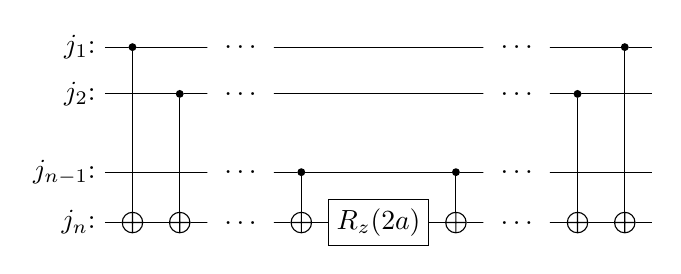
\begin{tikzpicture}
    \begin{yquant}
      qubit {$j_1\colon$} q[1];
      qubit {$j_2\colon$} q[+1];
      qubit {} q[+1]; discard q[2];
      qubit {$j_{n-1}\colon$} q[+1];
      qubit {$j_n\colon$} q[+1];
      cnot q[4] | q[0];
      cnot q[4] | q[1];
      text {$\ \ldots\ $} q[0,1,3,4];
      cnot q[4] | q[3];
      box {$R_z(2a)$} q[4];
      cnot q[4] | q[3];
      text {$\ \ldots\ $} q[0,1,3,4];
      cnot q[4] | q[1];
      cnot q[4] | q[0];
    \end{yquant}
  \end{tikzpicture}
  \fi
  \caption{Operaatori \(e^{-iZ_{j_1}Z_{j_2}\cdots Z_{j_n}a}\) realiseerimine kvantahelana~\cite{mansky+etal, nielsen+chuang}. Bitte, mis \(j_1\), \(j_2\), \(\cdots\), \(j_n\) hulgas ei esine, pole näidatud}
  \label{f:expz}
\end{figure}
Teisisõnu, bitile \(j_n\) tuleb järjest rakenda bittide \(j_1\), \(j_2\), \(\cdots\), \(j_{n-1}\) juhitud eitust.
Siis tuleb bitti \(j_n\) pöörata \(z\)-telje sihis nurga \(2a\) võrra.
Viimaks tuleb bitile \(j_n\) järjest rakendada bittide \(j_{n-1}\), \(j_{n-2}\), \(\cdots\), \(j_1\) juhitud eitusi.
Bitte, mis \(j_1\), \(j_2\), \(\cdots\), \(j_n\) hulgas ei esine, ei mõjutata.
Ahelat tuleks mõista nii, et kesksele väravale \(R_z(2a)\) eelnev juhitud eituste osa arvutab bittide \(j_1\), \(j_2\), \(\cdots\), \(j_n\) paarsuse, keskne värav \(R_z(2a)\) teeb sobiva pöörde ja järgnev juhitud eituste osa on paarsuse arvutamise pöördoperaatsioon.

Üldjuhul koosneb \(h_i\) nii Pauli \(I\) ja \(Z\) kui ka \(X\) ja \(Y\) operaatoritest, kuid \(h_i\) saab alati viia kujule~\eqref{eq:onlyz} rakendades sobivaid baasiteisendusi.
Vajalikud baasiteisendused on järgmised:
\begin{align}
    Z = HXH \rlap{,}\qquad Z = S^\dagger HYHS \rlap{.}
\end{align}
Näiteks juhul, kui
\begin{equation}
  h_i = Z_1X_2Y_3 \rlap{,}
\end{equation}
realiseerib operaatori \(e^{-i h_i t}\) ahel joonisel~\ref{f:xyzex}.

\begin{figure}[h]
  \centering
  \ifdefined\yquanton
  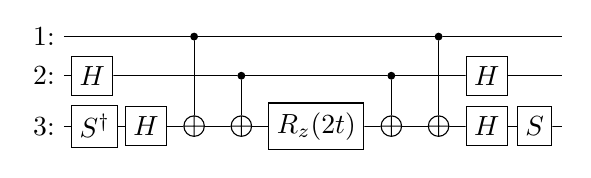
\begin{tikzpicture}
    \begin{yquant}
      qubit {$1\colon$} q[1];
      qubit {$2\colon$} q[+1];
      qubit {$3\colon$} q[+1];
      box {$H$} q[1];
      box {$S^{\dagger}$} q[2];
      box {$H$} q[2];
      cnot q[2] | q[0];
      cnot q[2] | q[1];
      box {$R_z(2t)$} q[2];
      cnot q[2] | q[1];
      cnot q[2] | q[0];
      box {$H$} q[1];
      box {$H$} q[2];
      box {$S$} q[2];
    \end{yquant}
  \end{tikzpicture}
  \fi
  \caption{Juhitud operaatori \(e^{-iZ_1X_2Y_3}\) realiseerimine kvantahelana.}
  \label{f:xyzex}
\end{figure}

Kokkuvõttes tuleb operaatori \(e^{-i t \sum_i h_i}\) realiseerimiseks kvantahelana gruppide kaupa järjestikku rakendada operaatoreid \(e^{-i h_i t/n}\) realiseerivaid kvantahelaid, kus \(n\) on piisavalt suur.
Näiteks, kui
\begin{align}\label{eq:hex}
    H=\frac{1}{3}X_1Y_1+\frac{2}{3}Z_1X_2 \rlap{,}
\end{align}
ja võtta trotterisammude arvuks \(n = 2\), siis realiseerib operaatori \(e^{-i Ht}\) ahel~\ref{fig:trot}.
Lõpliku trotterisammude arvu puhul on tegemist ligikaudse hinnanguga.

\begin{figure}
    \centering
    \ifdefined\yquanton
    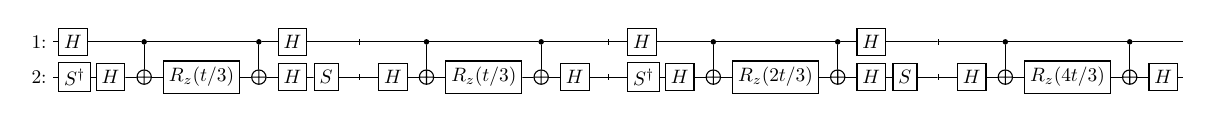
\begin{tikzpicture}[scale=0.7]
        \begin{yquant}
            qubit {$1\colon$} q[1];
            qubit {$2\colon$} q[+1];
            box {$H$} q[0];
            box {$S^\dagger$} q[1];
            box {$H$} q[1];
            cnot q[1] | q[0];
            box {$R_z(t/3)$} q[1];
            cnot q[1] | q[0];
            box {$H$} q[0];
            box {$H$} q[1];
            box {$S$} q[1];
            barrier q;
            box {$H$} q[1];
            cnot q[1] | q[0];
            box {$R_z(t/3)$} q[1];
            cnot q[1] | q[0];
            box {$H$} q[1];
            barrier q;
            box {$H$} q[0];
            box {$S^\dagger$} q[1];
            box {$H$} q[1];
            cnot q[1] | q[0];
            box {$R_z(2t/3)$} q[1];
            cnot q[1] | q[0];
            box {$H$} q[0];
            box {$H$} q[1];
            box {$S$} q[1];
            barrier q;
            box {$H$} q[1];
            cnot q[1] | q[0];
            box {$R_z(4t/3)$} q[1];
            cnot q[1] | q[0];
            box {$H$} q[1];
        \end{yquant}
    \end{tikzpicture}
    \fi
    \caption{Operaatori \(e^{-i\paren{\frac{1}{3}X_1Y_1+\frac{2}{3}Z_1X_2} t}\) realiseerimine kvantahelana.
    Joonisel on kaks operaatorite gruppi, mis vastab kahele trotterisammule.
    Igas grupis on omakorda kaks operaatorit}
    \label{fig:trot}
\end{figure}

\subsection{Juhitud ajalise arengu operaator}\label{sec:cu}

Faasihindamise jaoks on oluline, et unitaarne operaator oleks juhitud.
Juhitud ajalise arengu operaatori saab, kui seda realiseerivas kvantahelas asendada kõik pöörded juhitud pööretega.
Nõnda toiminud, sõltub iga Pauli sõne rakendamine sellest, mis on juhtkvantbiti olek.
Kui juhtkvantbitt on olekus \(\ket{0}\), pööre ei rakendu.
Et paarsuse arvutamine ja selle tagasi panemine on pöördoperatsioonid, siis kokkuvõttes antud Pauli sõne eksponent ei rakendu.
Kui juhtkvantbitt on olekus \(\ket{1}\) pööre rakendub ja rakendub ka Pauli sõne eksponent tervikuna.
Joonisel~\ref{fig:trotexctrl} on näide juhitud ajalise arengu operaatorist, kui hamiltoniaan on antud valemiga~\eqref{eq:hex}.

\begin{figure}[h]
    \centering
    \ifdefined\yquanton
    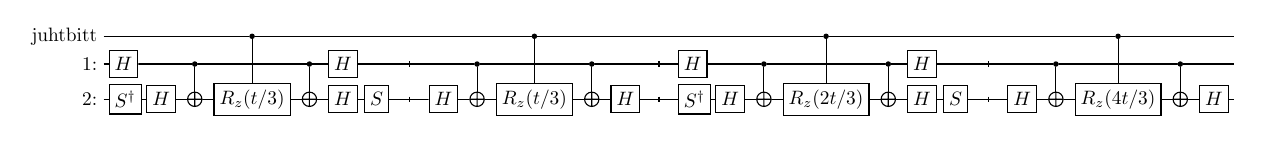
\begin{tikzpicture}[scale=0.7]
        \begin{yquant}
            qubit {juhtbitt} ctrl;
            qubit {$1\colon$} q[1];
            qubit {$2\colon$} q[+1];
            box {$H$} q[0];
            box {$S^\dagger$} q[1];
            box {$H$} q[1];
            cnot q[1] | q[0];
            box {$R_z(t/3)$} q[1] | ctrl[0];
            cnot q[1] | q[0];
            box {$H$} q[0];
            box {$H$} q[1];
            box {$S$} q[1];
            barrier q;
            box {$H$} q[1];
            cnot q[1] | q[0];
            box {$R_z(t/3)$} q[1] | ctrl[0];
            cnot q[1] | q[0];
            box {$H$} q[1];
            barrier q;
            box {$H$} q[0];
            box {$S^\dagger$} q[1] ;
            box {$H$} q[1];
            cnot q[1] | q[0];
            box {$R_z(2t/3)$} q[1] | ctrl[0];
            cnot q[1] | q[0];
            box {$H$} q[0];
            box {$H$} q[1];
            box {$S$} q[1];
            barrier q;
            box {$H$} q[1];
            cnot q[1] | q[0];
            box {$R_z(4t/3)$} q[1] | ctrl[0];
            cnot q[1] | q[0];
            box {$H$} q[1];
        \end{yquant}
    \end{tikzpicture}
    \fi
    \caption{Juhitud operaatori \(e^{-i\paren{\frac{1}{3}X_1Y_1+\frac{2}{3}Z_1X_2} t}\) realiseerimine kvantahelana.}
    \label{fig:trotexctrl}
\end{figure}

Kui hamiltoniaanis esineb liige, mis on vaid ühikmaatriksite tensorkorrutis, tuleb seda eraldi arvestada.
Sellise liikme eksponent on globaalse faasi operaator, mille võib mittejuhitud ajalise arengu operaatori juhul arvestamata jätta.
Samas juhitud globaalse faasi operaator rakendamine muudab suhtelist faasi ja seda peab arvestama.
Juhitud globaalse faasi operaatori võib asendanda juhtkvantbitil rakendatud suhtelise faasi operaatoriga, nagu näha joonisel~\ref{fig:globphase}, kus võrduse vasak ja parem pool on samaväärsed globaalse faasi täpsusega.

\begin{figure}[h]
    \centering
    \ifdefined\yquanton
    \begin{tikzpicture}
        \begin{yquantgroup}
            \registers{
                qubit {} q[2];
            }
            \circuit{
                box {\(GP(t)\)} q[1] | q[0];
            }
            \equals
            \circuit{
                box {\(P(-t)\)} q[0];
                barrier q[1];
            }
        \end{yquantgroup}
    \end{tikzpicture}
    \fi
    \caption{Juhitud globaalse faasi operaatori saab asendada juhtkvantbitile rakendatud faasi operaatoriga, mille argument peab olema vastupidine. Vasakul ja paremal pool olevate operaatorite mõju kvantregistrile on globaalse faasi täpsusega sama.}
    \label{fig:globphase}
\end{figure}

\section{Vahekokkuvõte}

Nüüdseks on meil olemas kõik osad põhienergia leidmise ülesande lahendamiseks.
Eelmise peatükis nägime, millised on vajalikud klassikalised eelarvutused~--- nende tulemuseks on hamiltoniaan teise kvantiseerimise kujul ja Hartree-Focki hinnang põhiolekule.
Selles peatükis nägime, kuidas see hamiltoniaan realiseerida kvantahelana, kasutades trotteriseerimist ja treppalgoritmi.
Samuti nägime selles peatükis, kuidas leida niiviisi realiseeritud hamiltoniaani omaväärtused, kui teada on huvipakkuvate omaolekute hinnangud.
Järgmises peatükis pöörame tähelepanu teoreetiliselt praktilisele.

\chapter{Metoodika ja tulemused}\label{chap:results}

Töö praktilises osas valmis programm molekulaarse süsteemi põhienergia leidmiseks.
Kõik selleks vajalikud kvantalgoritmid~--- kvantarvutuslik Fourier' teisendus ja pöördteisendus, faasi hindamine, treppalgoritm ja trotteriseerimine~--- implementeeriti iseseisvalt, lähtudes vaid primitiivsetest kvantväravatest.
Samuti implementeeriti iseseisvalt klassikaline algoritm faasi hindamise tulemuse väljalugemiseks.
Valmislahendusi kasutati vaid kvantkeemiliste eelarvutuste jaoks: molekulaarsete integraalide arvutamiseks ja Jordan-Wigneri teisenduseks.
Töö teoreetilises osas nägime, et faasi hindamine on universaalne meetod, kuivõrd seda saab kasutada mistahes molekuli mistahes taseme energia leidmiseks.
Sestap taotleti ka töö praktilises osas universaalsust, milleks oli vajalik ka programmi modulaarsus.
Praktilise osa tulemuseks on programm, mille osad on kapseldatud ja parametriseeritud: andes ette sobiva hamiltoniaani ja olekuvektori saab programmi kasutada soovitud molekuli soovitud energiataseme leidmiseks, kui muidugi arvutusvõimekus lubab.
Programmi testimiseks kasutati siiski konkreetset ülesannet.
Nimelt leiti \(\rm H_2\), lihtsaima võimaliku kaheaatomilise molekuli, põhienergia erinevatel sidemepikkustel.
Arvutused viidi läbi kasutades kvantarvuti klassikalist simulaatorit~--- seega  ei tekkinud vajadust töös käsitleda müra.

\section{Kasutatud vahendid ja lähtekood}

Töös kasutati läbivalt programmeerimiskeelt Python (versioon 30.10.12)~\cite{python}.
Kasutatud teegid on järgmised.
\begin{itemize}
  \item Molekulaarsete integraalide arvutamiseks ja Jordan-Wigneri teisenduseks~--- klassikalisteks eelarvutusteks kasutati teeki OpenFermion (versioon 1.6.1)~\cite{openfermion}, mis omakorda kasutas kvantkeemiaprogrammi Psi4~\cite{psi4}.
  \item Ahela koostamiseks kasutati teeki Qiskit (versioon 1.6.1)~\cite{qiskit}.
  \item Ahela simuleerimiseks kasutati olekuvektori simulaatorit teegist Qiskit Aer (vt eelmine punkt).
\end{itemize}
Arvuti kohta, mida kasutati kõikide arvutuste joaks, on oluline märkida järgnevat.
\begin{itemize}
  \item Protessor oli 32 tuumaga AMD Ryzen Threadripper 3970X.
  \item Arvutil oli \(256\,{\rm GB}\) mälu (lisaks swap-mälu \(135\,{\rm GB}\)).
  \item Arvutused toimusid operatsioonisüsteemil Ubuntu (versioon 22.04.4 LTS).
\end{itemize}
Kuigi programmil oli lubatud kasutada ka graafikakaarti NVIDIA A100, siis teegi Qiskit Aer sisemise heuristika tõttu see kasutust ei leidnud ja kõik arvutused viidi läbi protsessoril.
Koostatud programmi lähtekood on saadaval töö repositooriumis~\cite{repo}, kus on ka dokumenteeritud, kuidas programmi kasutada teegina või käsurealt.

\section{Metoodika}

Arvutati \(\rm H_2\) põhienergia erinevatel sidemepikkustel.
Lainefunktsiooni esitati keemilises baasis STO-3G, mis põhineb küll vaid kolmel reaalsel Gaussi funktsioonil, ent on siiski tihti praktikas piisavalt täpne~\cite{whitfield+etal2011, omalley+etal}}.
Selleks, et mõõtmistulemuste seast tõenäoliseim vastaks põhienergiale, tuleb enne faasi hindamist seisundiregistrisse tekitada olek, millel on suur kattuvus põhiolekuga.
Antud juhul kasutati põhiolekulähedast Hartree-Focki olekut
\begin{equation}
  \ket{\rm HF}=\ket{1100}\rlap.
\end{equation}
Arvutustes taotleti keemilist täpsust, nimelt seda, et arvutatud energia ei erineks võrdlusväärtusest rohkem kui \(\Delta E_{\rm chem}=1{,}6\,{\rm mHa}\).
Võrdlusväärtuseks loeti täieliku konfiguratsiooni vastasmõju meetodil arvutatu\footnote{Selle võimaldas arvutada teek OpenFermion.}, kuivõrd tegemist on klassikaline meetodiga, mis annab nii täpse tulemuse, kui keemiline baas lubab~\cite{mcardle+etal}.
Energiaid otsiti ülemise piiri \(E_h=1\,{\rm Ha}\) ja alumise piiri \(E_l=-2\,{\rm Ha}\) vahelt~--- skaleerimiskonstant oli \(t={1\over E_h-E_l}\).
Faasi hindamise parameeter $N$, mis on täpsusbittide arv, leiti kriteeriumi
\begin{equation}
  \Delta E_{\rm chem}t\ge 2^{-N-1}
\end{equation}
põhjal.
Teisisõnu, nõuti, et faasi hindamise viga poleks suurem keemilisest täpsusest.
Antud juhul oli $N=11$.
Trotterisammude arv leiti eksperimentaalselt, proovides järjest suuremat sammude arvu, kuni viga muutus keemilisest täpsusest väiksemaks.
Arvutati energiad sidemepikkustel \(0{,}2\ldots 3\,{\rm Å}\).

\section{Tulemused}

Töö tulemused võtab kokku joonis~\ref{fig:h2plots}, mille kohta käivad järgmised tähelepanekud.

\begin{figure}
  \centering
  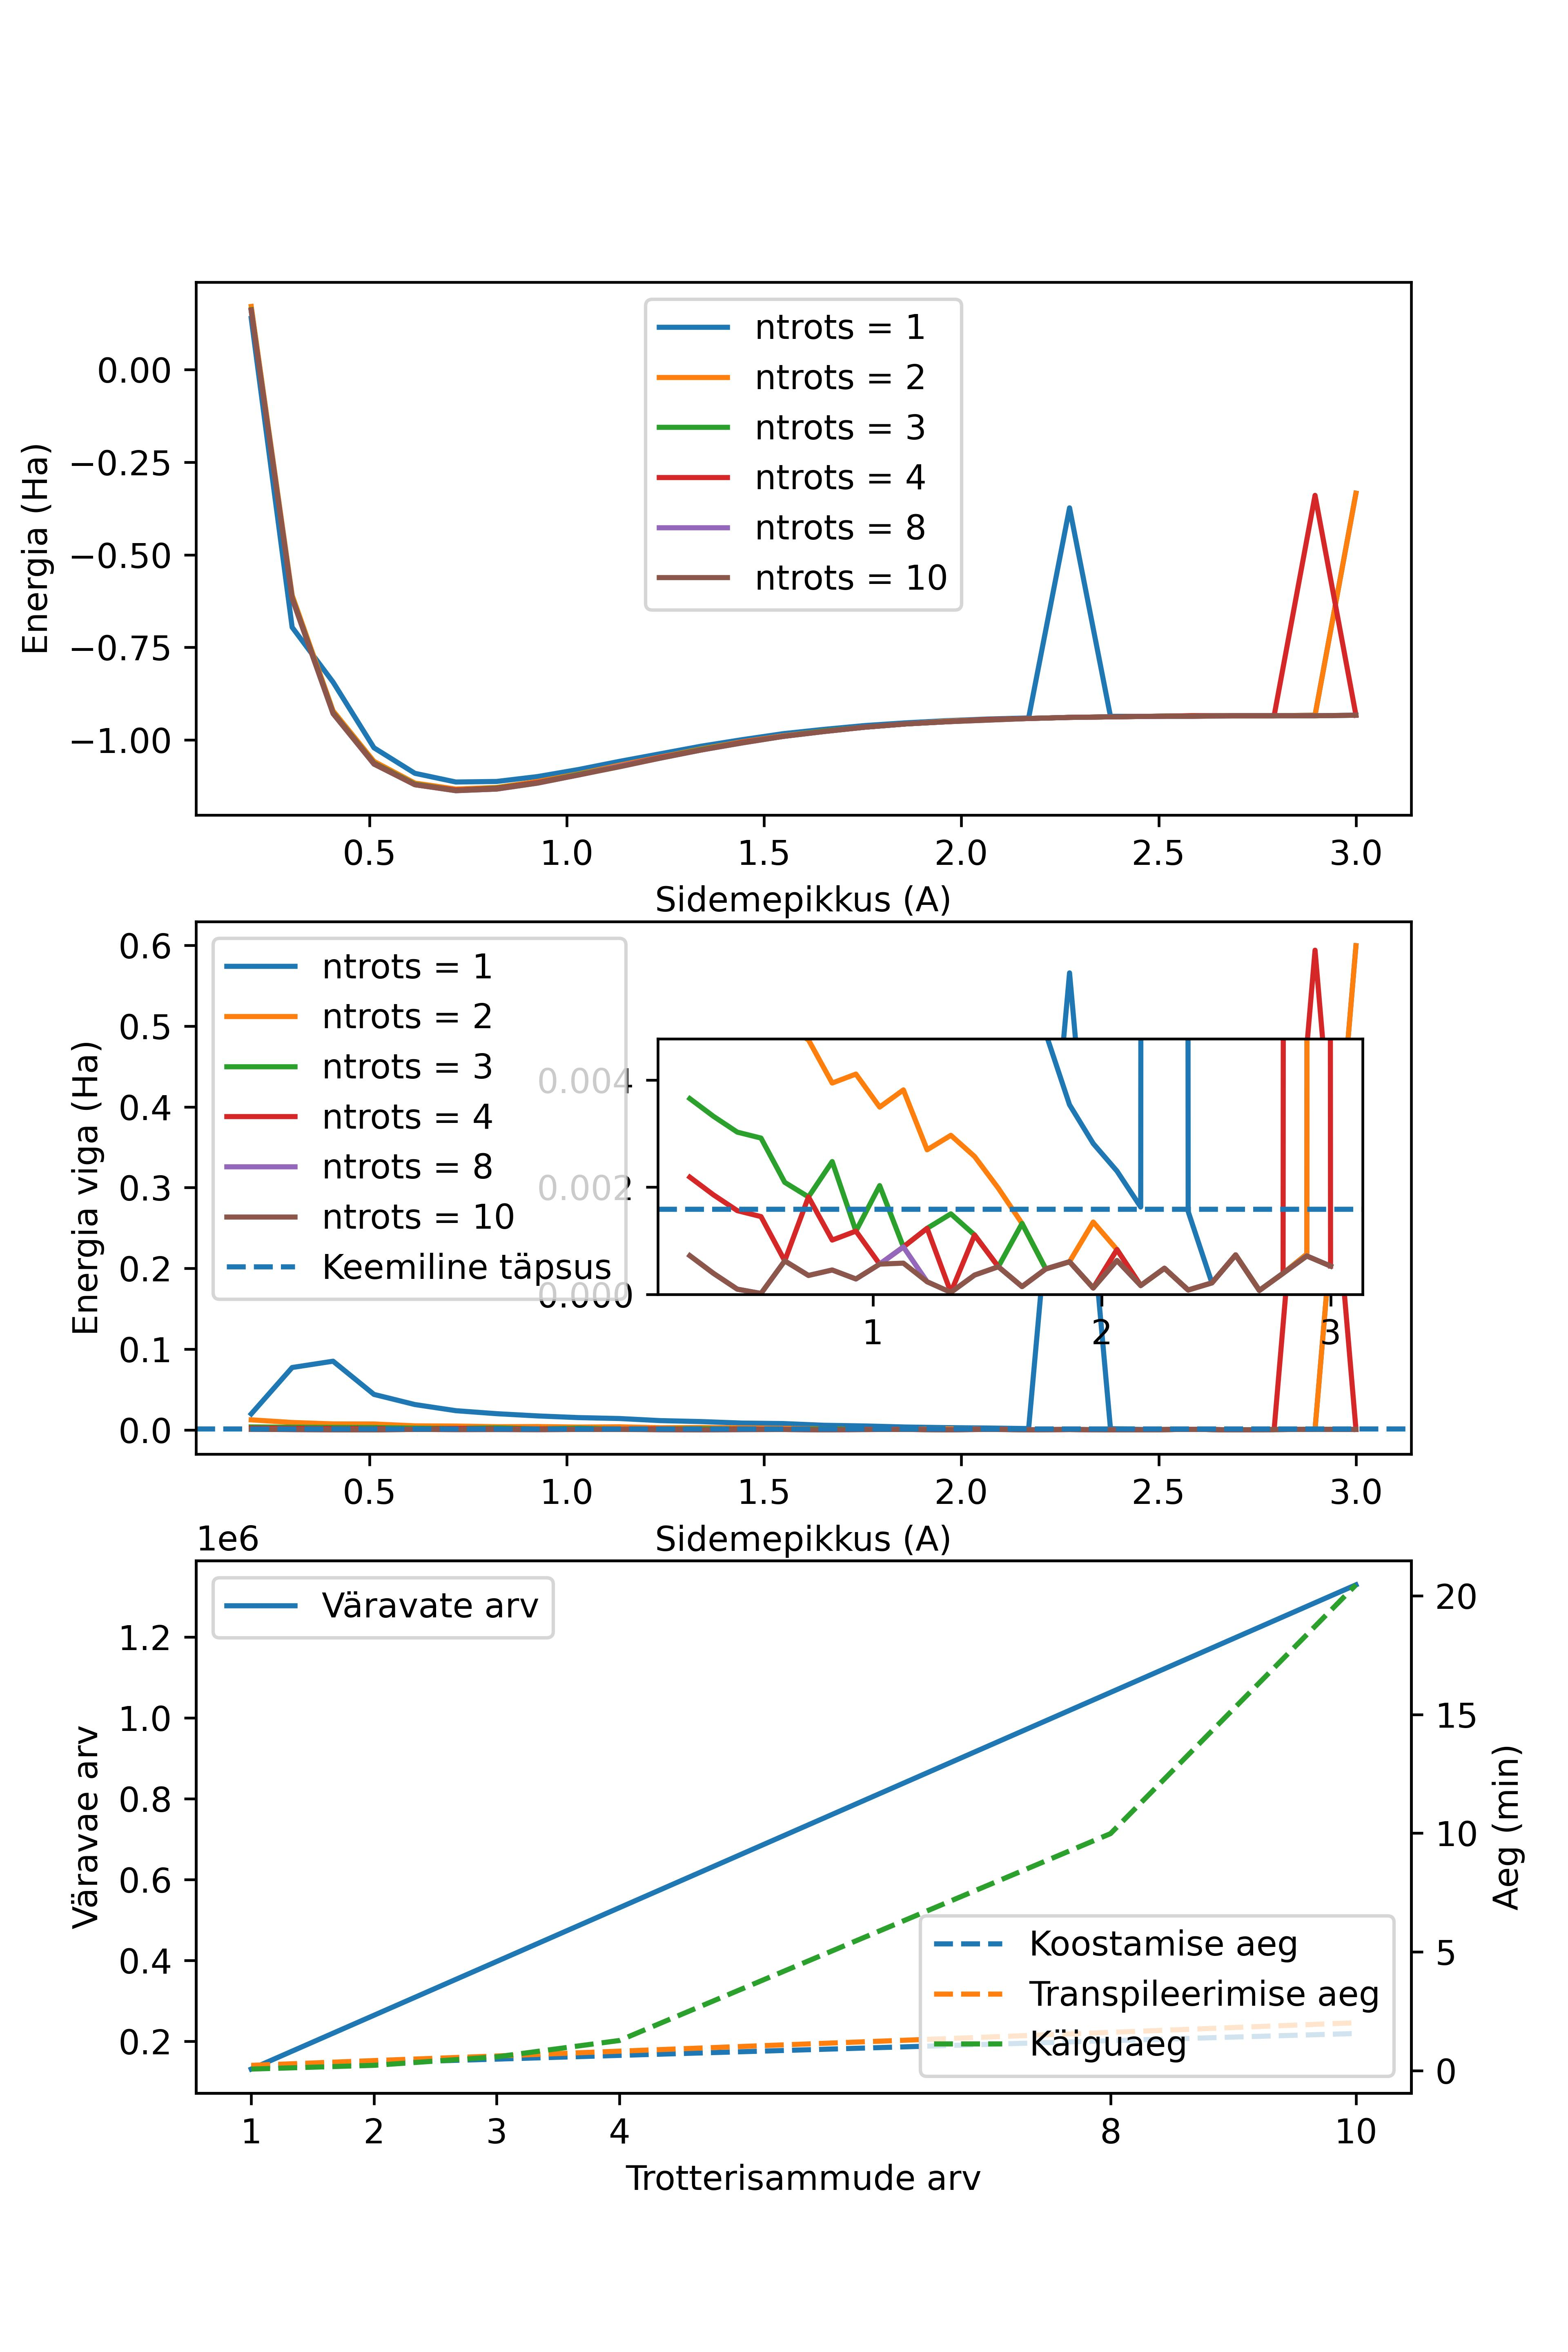
\includegraphics[height=.75\vsize]{h2plots.jpg}
  \caption{Üleval: energia sõltuvus sidemepikkusest erinevate trotterisammude arvude jaoks.
    Keskel: energia vea sõltuvus sidemepikkusest erinevate trotterisammude arvude jaos.
    Nii üleval kui ka keskel on kaheksale trotterisammule, mis on antud ülesandes keemilise täpsuse jaoks piisav, vastav sõltuvus esitatud rõhutatult punktidega joonega.
    All: ahela väravate arvu sõltuvus trotterisammude arvust (vasakpoolne vertikaaltelg, pidevjoon); koostamiseks, kompileerimiseks ja käitamiseks kulunud aegade sõltuvus trotterisammude arvust (parempoolne vertikaaltelg, katkendjoon).}
  \label{fig:h2plots}
\end{figure}

Ülemisel paneelil on a energia sõltuvus sidemepikkusest.
Juhul, kui trotterisammude arv on piisav, on sõltuvus selline, nagu võiks füüsikalistel kaalutlustel oodata: energial on üksainus negatiivse väärtusega miinimum.
Miinimum vastab tasakaalugeomeetriale, mille puhul on sidemepikkus \(\apporx0{,}75\,{\rm Å}\).

Keskmisel paneelil on kujutatud, kuidas sõltub energiaviga trotterisammude arvust ja sidemepikkusest.
Energiavea all peame silmas leitud energia erinevust võrdlusväärtusest.
Energiavea alaliik on tortteriviga: s.o viga, mis tuleneb lõplikust tortterisammude arvust.
Keskmiselt paneelilt võib välja lugeda, et trotteriviga on kõikide sidemepikkust jaoks väiksem keemilisest täpsusest alles siis, kui trotterisammude arv on vähemalt \(8\).
Üldine tendents on, et trotteriviga on seda suurem, mida lühem on sidemepikkus.
% Selline käitumine on põhjendatav: lühem sidemepikkus tähendab suuremat interaktsiooni ja interaktsiooniga on seotud just need liikmed, mis panustavad trotterivikka.
% Teisisõnu, kui hamiltoniaan koosneks vaid kommuteeruvatest liikmetest, mis oleks tõsi lõpmatu sidemepiikkuse juures, siis trotteriviga ei esineks.

Alumine paneel on ahela arvutusliku kulukuse kohta.
Selgub, et väravate arv sõltub trotterisammude arvust lineaarselt.
Samas ahela klassikalise simuleerimise käiguaeg sõltub trotterisammude arvust eksponentsiaalselt, jõudes \(10\) trotterisammu juures \(20\,{\rm min}\).
% Viimasest kahest väitest nähtub, et kvantahelat klassikaliselt simuleerides ei ole võimalik saavutada seda ajavõitu, mida kvantalgortm muidu klassikalise ees võimaldab.
Lisaks on alumiselt paneelilt näha, et ka ahela koostamise ja kompileerimise ajad pole tühised.

Tööd võib lugeda kordaläinuks, kuivõrd töös kirjeldatud meetodil on tõepoolest võimalik arvutad \(\rm H_2\) põhioleku energia.
Nagu varem mainitud, saaks sama meetodit kasutad ka teiste molekulide ja kõrgemate tasemete energiate arvutamiseks, ent antud töös takistas selle tegemist vajadus kvantarvutit klassikaliselt simuleerida.
Viise, kuidas siiski keerulisemaid süsteeme uurida, käsitleb järgmine alapeatükk.

\section{Kvantarvutuse hetkeseis ja võimalikke edasiarendusi}

Faasi hindamise näol on tegemist algoritmiga, mis eeldab loogiliste kvantbittide kasutamise võimalust~--- öeldakse, et tegemist on veatolerantse algoritmiga.
Loogilised kvantbitid on sellised, milles on müra piisavalt alla surutud, et oleks võimalik läbi viia pikki arvutusi, mis praktikas ette tulevad.
Et füüsikalised kvantbitid~--- need, mis on riistvaras päriselt olemas~--- on alati mürarikkad, tuleb loogilised kvantbitid realiseerida suure arvu füüsikaliste kvantbittide kaudu.
Töö kirjutamise ajal ei ole universaalseks kasutamiseks loogilisi kvantbitte suudetud realiseerida.
Seega on kvantarvutite kasutamine päris arvutusteks olnud piiratud vaid nendele ülesannetele, mida on võimalik lahendada vaatamata märkimisväärsele müratasemele.
Praeguse periood kohta kasutatakse lühendit NISQ (ingl noisy intermediate-scale quantum)~\cite{preskill}.
Mõistagi soovitakse jõua järgmisesse perioodi, kus neid puuduseid pole, mille kohta kasutatakse lühendit FTQC (ingl fault-tolerant quantum computing).
Kvantarvutite riistvara arendamisega tegelevad ettevõtted ja uurimisasutused on võtnud eesmärgiks jõuda 2020ndate aastate lõpuks selle perioodi lävele~\cite{ibmq+roadmap, quera+roadmap}.
Esimesed sammud selle eesmärgi suunas on juba tehtud: Quera töörühmal õnnestus realiseerida 48 loogilist kvantbitti mõnede arvutuste jaoks~\cite{quera}.
Siin töös esitatud viisil vesiniku molekuli põhienergia arvutamiseks keemilise täpsusega oleks vaja kvantarvutit, millel on \(11 + 4\) loogilist kvantbitti.
Töö tegijale selliste kvantarvutit kasutada polnud, mis motiveerib uurima töös esitatud lahendamisskeemi võimalikke edasiarendusi, mida oleks võimalik rakendada ka kasinamate vahenditega.

Põhisuunad selleks on järgmised.
\begin{itemize}
  \item Faasihindamise asemel saab kasutada algoritmi, mis pole müra suhtes niivõrd tundlik: selline on näiteks variatsioonilise lahendamise kvantalgoritm~\cite{omalley+etal, raidlo}.
  \item Faasihindamise algoritmi saab teha iteratiivseks, mis lubab faasi hindamise algoritmi ahela asemel käitada rida lühemaid ja vähemate kvantbittidega ahelaid, mida tuleb koordineerida klassikaliste arvutuste abil~\cite{whitfield+etal2011, omalley+etal}.
  \item Hamiltoniaani saab ressursside kokkuhoidmiseks lihtsustada, nagu on seda teinud näiteks O'Malley jt~\cite{omalley+etal}.
\end{itemize}
Siin esitatud lahendamisskeem on siiski võimalikest edasiarendustest üldisem, mis õigustab antud töös sellele pööratud tähelepanu.

\chapter{Kokkuvõte}

Töös leiti molekulaare süsteemi põhienergia kasutades kvantarvutusliku meetodit.
Selleks vajalik teooria esitati lähtudes alustõdedest, kusjuures erilist tähelepanu pöörati kvantarvutuslikule osale.

Esmalt käsitletigi elektronstruktuuri ülesande teoreetilist tausta.
Alustati molekulaarse süsteemi üldisest hamiltoniaanist.
Käsitlust lihtsustati kasutades kõigepealt Born-Oppenheimeri ja hiljem Hartree-Focki lähendust.
Olekud esitati Slateri determinandina.
Viidi läbi teine kvantiseerimine, mis oli vajalik töö järgmises osas, st ülesande kodeerimisel kvantarvutil lahendamiseks.

Järgmisena esitati hamiltoniaan ja olekud kvantbittide ruumis kasutades Jordan-Wigneri teisendust.
Saadud Pauli sõnedest hamiltoniaani põhjal koostati kvantahel kasutades trotteriseerimist ja treppalgoritmi.

Edasi tutvustati faasi hindamise algoritmi kui meetodit kvantbittide ruumis esitatud hamiltoniaani omaolekute energiate leidmiseks.
Näidati, et faasi hindamine taandub kvantarvutusliku Fourier' teisenduse ja pöördteisenduse tegemisele.
Samuti näidati, kuidas hamiltoniaani omaväärtust sobivalt skaleerida, et see oleks võimalik välja lugeda faasist, mis on perioodiline.

Töö praktilises osas koostati teoreetilise osa tulemuste põhjal programm, millega arvutati \(\rm H_2\) põhienergia.
Arvutused viidi läbi kvantarvuti klassikalisel simulaatoril.
Tulemusi võrreldi täieliku konfiguratsiooni vastasmõju meetodil arvutatutega.
Leiti, et töös esitatud meetod on tõepoolest ülesande lahendamiseks sobiv.

Lõpuks käsitleti töö võimalik edasiarendusi, st seda, kuidas oleks võimalik antud ülesannet lahendada juba praegu, NISQ perioodil.

\printbibliography[heading=bibintoc, title=Kirjandus]

\end{document}
